\documentclass[11pt,letter]{article}
\pdfoutput=1
\usepackage{jheppub}
\usepackage{amsmath,amssymb}
\usepackage[dvipsnames]{xcolor}
%\usepackage{hyperref}
\usepackage{xspace}
\usepackage{ifdraft}
\usepackage{epstopdf}
\usepackage{slashed}
\usepackage{anyfontsize}
\usepackage{tocloft}
\renewcommand{\cftdot}{.}
\renewcommand{\cftsubsecleader}{\cftdotfill{\cftdotsep}}
\usepackage{diagbox}
\usepackage{colortbl}
\usepackage{bbold}
\usepackage{tabularx}
\usepackage{graphicx}
\usepackage{stackengine}
\usepackage{subcaption}
\usepackage{cleveref}
\usepackage[normalem]{ulem}

\def\RA{\rlap{\scalebox{1.6}{$\leftrightarrow$}}}
\def\DA{\smash{\bclap{\scalebox{1.6}{$\downarrow$}}}}
\def\mystrut{\rule[-2ex]{0ex}{6ex}}

\usepackage{tikz-feynman} 

%%%%%%%%%%%%%%%%%%%%%%%%%%%%%%%%%%%%%%%%%%%
% Comment the following out to compile new images

\usetikzlibrary{external}  
\immediate\write18{mkdir -p images}  %% Create `pgf-img` directory
\tikzexternalize[                     %% Activate externalization
prefix=images/,                    %% Avoid cluttering the directory
system call={                       %% Use lualatex in system call
   pdflatex \tikzexternalcheckshellescape -halt-on-error -shell-escape -interaction=batchmode -jobname="\image" "\texsource" || rm "\image.pdf"
},
]
%%%%%%%%%%%%%%%%%%%%%%%%%%%%%%%%%%%%%%%%%%%


\usepackage[notcite]{showkeys}
\usepackage{tikz-feynman} 
\usepackage{xcolor}
\hypersetup{
    colorlinks,
    linkcolor={nhpRed},
    citecolor={nhpBlue},
    urlcolor={nhpBlue}
}


\definecolor{nhpRed}{RGB}{161,0,0}
\definecolor{nhp4}{RGB}{203, 4, 31}
\definecolor{nhp3}{RGB}{244,99,30}
\definecolor{nhp2}{RGB}{255,159,0}
\definecolor{nhp1}{RGB}{48,152,152}
\definecolor{nhpBlue}{RGB}{0,100,144}
\definecolor{cutred}{RGB}{219,56,49}
\definecolor{hgreen}{RGB}{25,176,146}
\definecolor{hgreen1}{RGB}{175,230,175}
\definecolor{hblue}{RGB}{52,152,219}
\definecolor{hbluedark}{RGB}{36, 106, 160}
\definecolor{hblue1}{RGB}{255,255,166}
\definecolor{hred}{RGB}{216,83,117}
\definecolor{hreddark}{RGB}{151, 58, 81}
\definecolor{hred1}{RGB}{255,155,155}
\definecolor{cutred}{RGB}{219,56,49}
\definecolor{hgrey4}{RGB}{75,75,75}
\definecolor{hgrey5}{RGB}{50,50,50}
\definecolor{hgrey3}{RGB}{100,100,100}
\definecolor{hgrey}{RGB}{125,125,125}
\definecolor{hgrey2}{RGB}{125,125,125}
\definecolor{hgrey1}{RGB}{150,150,150}
\definecolor{hgrey0}{RGB}{175,175,175}
\definecolor{darkgreen}{RGB}{59,126,108}
\definecolor{nu-80}{RGB}{104, 076, 150}
\definecolor{nu-40}{RGB}{164, 149, 195}
\colorlet{ucp-color}{nhpBlue}
\colorlet{cut-color}{nhp4}
\colorlet{jacobi-color}{nhp4}
\colorlet{refl-color}{nhp4}


%Comment commands
\newcommand{\ace}[1]{\textcolor{darkgreen}{\textbf{AE:}{ #1}}}
\newcommand{\nhp}[1]{\textcolor{nhpRed}{\textbf{NHP:}{#1}}}
\newcommand{\jm}[1]{\textcolor{blue}{\textbf{JM: }{#1}}}


\usepackage[framemethod=default]{mdframed}
\newmdenv[skipabove=7pt,
skipbelow=7pt,
rightline=false,
leftline=false,
topline=false,
bottomline=false,
backgroundcolor=gray!15,
linecolor=gray,
innerleftmargin=5pt,
innerrightmargin=5pt,
innertopmargin=5pt,
innerbottommargin=5pt,
leftmargin=0cm,
rightmargin=0cm,
linewidth=4pt]{eBox}


% TIKZ preamble and setup for external runs
\usetikzlibrary{calc}
\tikzset{Bfield/.style={decorate, double}}


%Code for externalizing the tikz image generations
\iffalse
\tikzfeynmanset{compat=1.1.0}
\immediate\write18{mkdir -p images}  %% Create `pgf-img` directory
\usetikzlibrary{external}  
          %% Load the `external` library
\immediate\write18{mkdir -p images}  %% Create `pgf-img` directory
\tikzexternalize[                     %% Activate externalization
  prefix=images/,                    %% Avoid cluttering the directory
 system call={                       %% Use lualatex in system call
    pdflatex \tikzexternalcheckshellescape -halt-on-error -shell-escape -interaction=batchmode -jobname="\image" "\texsource" || rm "\image.pdf"
  },
]
\fi

%Style definitions
\tikzfeynmanset{
  fermion2/.style={
    /tikz/postaction={
      /tikz/decoration={
        markings,
        mark=at position 0.7 with {
          \arrow{>[length=6pt, width=7pt]};
        },
      },
      /tikz/decorate=true,
    },
  },
}

% Put the baseline at the center of the picture, for every
% picture. The shift makes it closer to being centered in the center
% of the line (for intance with equations) rather than the center
% sitting on the baseline itself (which in equations makes things look
% not-centered against operators)
\tikzset{every picture/.style={baseline={([yshift=-.7ex]current bounding box.center)}}}

% Diagram definitions

%% Nice blob definition consistent with what James was already using,
%% but handling the coordinate duplication internally.
\newcommand{\blob}[2]{\vertex[dot,scale=2] (#1) at (#2){};\vertex[dot,scale=1.5,hgrey0] at (#2){};}
%% Use the same syntax, so that it is easy to convert between blobby
%% cuts and normal diagrams
\newcommand{\ver}[2]{\coordinate (#1) at (#2){};}



\newcommand{\KTDBContrib}[4]{ {
    \begin{tikzpicture}
      \pgfmathsetmacro{\cutlength}{0.8}
\begin{feynman}
\vertex (a1) at (-1.5,1){#4};
\vertex (a2) at (1.5,-1){#2};
\vertex (a3) at (1.5,1){#3};
\vertex (a4) at (-1.5,-1){#1};
\vertex (mid1) at (0,-.5);
\vertex (mid2) at (0,.5);
\vertex (mid3) at (1,.5) ;
\vertex (mid4) at (1,-.5) ;
\vertex (mid5) at (-1,.5);
\vertex (mid6) at (-1,-.5) ;
% Cut reference coords at the center of each line
%LH box midpoints
\vertex (m1) at ($(mid5)!0.5!(mid6)$);
\vertex (m2) at ($(mid1)!0.5!(mid6)$);
\vertex (m3) at ($(mid5)!0.5!(mid2)$);
\vertex (clo) at ($(m2)!0.5!(m3)$) {};
\vertex (c1) at ($(clo)+(90:\cutlength)$);
\vertex (c2) at ($(clo)+(180:\cutlength)$);
\vertex (c3) at ($(clo)+(270:\cutlength)$);
%RH box midpoints
\vertex (m4) at ($(mid3)!0.5!(mid4)$);
\vertex (m5) at ($(mid3)!0.5!(mid2)$);
\vertex (m6) at ($(mid4)!0.5!(mid1)$);
\vertex (cro) at ($(m5)!0.5!(m6)$) {};
\vertex (c4) at ($(cro)+(90:\cutlength)$);
\vertex (c5) at ($(cro)+(0:\cutlength)$);
\vertex (c6) at ($(cro)+(270:\cutlength)$);


\diagram{
(a4) --[ultra thick,](mid6),
(a3) --[ultra thick,](mid3),
(a2) --[ultra thick,](mid4),
(a1) --[ultra thick,](mid5),
(mid1) --[ultra thick,ucp-color](mid2),
(mid3) --[ultra thick,](mid2),
(mid1) --[ultra thick,](mid6),
(mid1) --[ultra thick,](mid4),
(mid5) --[ultra thick,](mid2),
(mid5) --[ultra thick,](mid6),
(mid3) --[ultra thick,](mid4),
(clo)--[ultra thick,dashed,blue](c1),
(clo)--[ultra thick,dashed,blue](c2),
(clo)--[ultra thick,dashed,blue](c3),
(cro)--[ultra thick,dashed,blue](c4),
(cro)--[ultra thick,dashed,blue](c5),
(cro)--[ultra thick,dashed,blue](c6)
};
\end{feynman}
\end{tikzpicture}
}
}


%%% Jacobi 1 %%%

\newcommand{\JacobiOneDoubleBox}{ {
\begin{tikzpicture}
\begin{feynman}
\vertex (a1) at (-1.5,1){4};
\vertex (a2) at (1.5,-1){2};
\vertex (a3) at (1.5,1){3};
\vertex (a4) at (-1.5,-1){1};
\vertex (mid1) at (0,-.5);
\vertex (mid2) at (0,.5);
\vertex (mid3) at (1,.5) ;
\vertex (mid4) at (1,-.5) ;
\vertex (mid5) at (-1,.5);
\vertex (mid6) at (-1,-.5) ;
\diagram{
(a4) --[ultra thick,](mid6),
(a3) --[ultra thick,](mid3),
(a2) --[ultra thick,](mid4),
(a1) --[ultra thick,](mid5),
(mid1) --[ultra thick,](mid2),
(mid3) --[ultra thick,](mid2),
(mid1) --[ultra thick,](mid6),
(mid1) --[ultra thick,](mid4),
(mid5) --[ultra thick,nhp4](mid2),
(mid5) --[ultra thick,](mid6),
(mid3) --[ultra thick,](mid4),
};
\end{feynman}
\end{tikzpicture}
}
}

\newcommand{\JacobiOneCrossedBox}{ {
\begin{tikzpicture}
\begin{feynman}
\vertex (a1) at (-1.5,1){4};
\vertex (a2) at (1.5,-1){2};
\vertex (a3) at (1.5,1){3};
\vertex (a4) at (-1.5,-1){1};
\vertex (mid1) at (0,-.5);
\vertex (mid2) at (0,.5);
\vertex (mid3) at (1,.5);
\vertex (mid4) at (1,-.5);
\vertex (mid5) at (-1,.5);
\vertex (mid6) at (-1,-.5);
\vertex (mid7) at (-.5,0) {};
\diagram{
(a4) --[ultra thick,](mid6),
(a3) --[ultra thick,](mid3),
(a2) --[ultra thick,](mid4),
(a1) --[ultra thick,](mid5),
(mid1) --[ultra thick,](mid6),
(mid3) --[ultra thick,](mid2),
(mid1) --[ultra thick,](mid4),
(mid5) --[ultra thick,](mid7),
(mid7) --[ultra thick,](mid1),
(mid2) --[ultra thick,](mid6),
(mid5) --[ultra thick,nhp4](mid2),
(mid3) --[ultra thick,](mid4),
};
\end{feynman}
\end{tikzpicture}
}
}

\newcommand{\JacobiOnePentaTriangle}{ {
\begin{tikzpicture}
\begin{feynman}
\vertex (a1) at (-1.5,1){4};
\vertex (a2) at (.5,-1){2};
\vertex (a3) at (.5,1){3};
\vertex (a4) at (-1.5,-1){1};
\vertex (mid1) at (-.5,-.5);
\vertex (mid2) at (-1,0);
\vertex (mid3) at (0,.5) ;
\vertex (mid4) at (0,-.5) ;
\vertex (mid5) at (-1,.5);
\vertex (mid6) at (-1,-.5) ;
\diagram{
(a4) --[ultra thick,](mid6),
(a3) --[ultra thick,](mid3),
(a2) --[ultra thick,](mid4),
(a1) --[ultra thick,](mid5),
(mid1) --[ultra thick,](mid2),
(mid6) --[ultra thick,](mid2),
(mid1) --[ultra thick,](mid6),
(mid1) --[ultra thick,](mid4),
(mid5) --[ultra thick,](mid3),
(mid5) --[ultra thick,nhp4](mid2),
(mid3) --[ultra thick,](mid4),
};
\end{feynman}
\end{tikzpicture}
}
}

%%% Jacobi 1 end %%%

%%% Jacobi 2 start %%%

\newcommand{\JacobiTwoCrossedBoxOne}{ {
\begin{tikzpicture}
\begin{feynman}
\vertex (a1) at (-1.5,1){2};
\vertex (a2) at (1.5,-1){4};
\vertex (a3) at (1.5,1){3};
\vertex (a4) at (-1.5,-1){1};
\vertex (mid1) at (0,-.5);
\vertex (mid2) at (0,.5);
\vertex (mid3) at (1,.5);
\vertex (mid4) at (1,-.5);
\vertex (mid5) at (-1,.5);
\vertex (mid6) at (-1,-.5);
\vertex (mid7) at (-.5,0) {};
\diagram{
(a4) --[ultra thick,](mid6),
(a3) --[ultra thick,](mid3),
(a2) --[ultra thick,](mid4),
(a1) --[ultra thick,](mid5),
(mid1) --[ultra thick,](mid6),
(mid3) --[ultra thick,](mid2),
(mid1) --[ultra thick,nhp4](mid4),
(mid5) --[ultra thick,](mid7),
(mid7) --[ultra thick,](mid1),
(mid2) --[ultra thick,](mid6),
(mid5) --[ultra thick,](mid2),
(mid3) --[ultra thick,](mid4),
};
\end{feynman}
\end{tikzpicture}
}
}

\newcommand{\JacobiTwoCrossedBoxTwo}{ {
\begin{tikzpicture}
\begin{feynman}
\vertex (a1) at (-1.5,1){3};
\vertex (a2) at (1.5,-1){4};
\vertex (a3) at (1.5,1){1};
\vertex (a4) at (-1.5,-1){2};
\vertex (mid1) at (0,-.5);
\vertex (mid2) at (0,.5);
\vertex (mid3) at (1,.5);
\vertex (mid4) at (1,-.5);
\vertex (mid5) at (-1,.5);
\vertex (mid6) at (-1,-.5);
\vertex (mid7) at (-.5,0) {};
\diagram{
(a4) --[ultra thick,](mid6),
(a3) --[ultra thick,](mid3),
(a2) --[ultra thick,](mid4),
(a1) --[ultra thick,](mid5),
(mid1) --[ultra thick,](mid6),
(mid3) --[ultra thick,](mid2),
(mid1) --[ultra thick,nhp4](mid4),
(mid5) --[ultra thick,](mid7),
(mid7) --[ultra thick,](mid1),
(mid2) --[ultra thick,](mid6),
(mid5) --[ultra thick,](mid2),
(mid3) --[ultra thick,](mid4),
};
\end{feynman}
\end{tikzpicture}
}
}

\newcommand{\JacobiTwoCrossedBoxThree}{ {
\begin{tikzpicture}
\begin{feynman}
\vertex (a1) at (-1.5,1){1};
\vertex (a2) at (1.5,-1){4};
\vertex (a3) at (1.5,1){2};
\vertex (a4) at (-1.5,-1){3};
\vertex (mid1) at (0,-.5);
\vertex (mid2) at (0,.5);
\vertex (mid3) at (1,.5);
\vertex (mid4) at (1,-.5);
\vertex (mid5) at (-1,.5);
\vertex (mid6) at (-1,-.5);
\vertex (mid7) at (-.5,0) {};
\diagram{
(a4) --[ultra thick,](mid6),
(a3) --[ultra thick,](mid3),
(a2) --[ultra thick,](mid4),
(a1) --[ultra thick,](mid5),
(mid1) --[ultra thick,](mid6),
(mid3) --[ultra thick,](mid2),
(mid1) --[ultra thick,nhp4](mid4),
(mid5) --[ultra thick,](mid7),
(mid7) --[ultra thick,](mid1),
(mid2) --[ultra thick,](mid6),
(mid5) --[ultra thick,](mid2),
(mid3) --[ultra thick,](mid4),
};
\end{feynman}
\end{tikzpicture}
}
}


%%% Jacobi 2 end %%%

%%% Graph sym start %%%

\newcommand{\CrossedBoxGraphSym}{ {
\begin{tikzpicture}
\begin{feynman}
\vertex (a1) at (-1.5,1){};
\vertex (a2) at (1.5,-1){};
\vertex (a3) at (1.5,1){};
\vertex (a4) at (-1.5,-1){};
\vertex (mid1) at (0,-.5);
\vertex (mid2) at (0,.5);
\vertex (mid3) at (1,.5);
\vertex (mid4) at (1,-.5);
\vertex (mid5) at (-1,.5);
\vertex (mid6) at (-1,-.5);
\vertex (mid7) at (-.5,0) {};
\vertex (x1) at (-1.5,0);
\vertex (x2) at (1.5,0);
\diagram{
(a4) --[ultra thick,](mid6),
(a3) --[ultra thick,](mid3),
(a2) --[ultra thick,](mid4),
(a1) --[ultra thick,](mid5),
(mid1) --[ultra thick,](mid6),
(mid3) --[ultra thick,](mid2),
(mid1) --[ultra thick,](mid4),
(mid5) --[ultra thick,](mid7),
(mid7) --[ultra thick,](mid1),
(mid2) --[ultra thick,](mid6),
(mid5) --[ultra thick,](mid2),
(mid3) --[ultra thick,](mid4),
(x1) --[ultra thick,dashed,nhp4](x2),
};
\end{feynman}
\end{tikzpicture}
}
}

%%% Graph sym end %%%

%%% Unitarity cuts begin %%%

\newcommand{\PhysicalCutOne}[4]{ {
\begin{tikzpicture}[baseline=6]
\begin{feynman}
\vertex (a1) at (-1, 1) {#1};
\vertex (a2) at (1, 1) {#2};
\vertex [dot,scale=2](mid1) at (0.5,0.5){};
\vertex [dot,scale=1.5,hgrey0](mid2) at (0.5,0.5){};
\vertex [dot,scale=2](mid3) at (-0.5,0.5){};
\vertex [dot,scale=1.5,hgrey0](mid4) at (-0.5,0.5){};
\vertex [dot,scale=2](mid5) at (0,0){};
\vertex [dot,scale=1.5,hgrey0](mid6) at (0,0){};
\vertex (a3) at (-.5, -.5) {#3};
\vertex (a4) at (.5, -.5) {#4};
\diagram{
(mid3) --[ ultra thick](a1),
(mid1) --[ ultra thick](a2),
(mid1) --[ ultra thick,out=120,in=60,min distance=0.1cm](mid3),
(mid1) --[ ultra thick](mid3),

(mid1) --[ ultra thick](mid5),
(mid3) --[ ultra thick](mid5),

(mid5) --[ ultra thick](a4),
(mid5) --[ ultra thick,](a3)
};
\end{feynman}
\end{tikzpicture}
}
}

\newcommand{\PhysicalCutTwo}[4]{ {
\begin{tikzpicture}
\begin{feynman}
\vertex (a1) at (-.6, -0.6) {#1};
\vertex (a2) at (-.6, 0.6) {#2};
\vertex [dot,scale=2](mid1) at (0,0){};
\vertex [dot,scale=1.5,hgrey0](mid2) at (0,0){};
\vertex [dot,scale=2](mid3) at (.8,0){};
\vertex [dot,scale=1.5,hgrey0](mid4) at (.8,0){};
\vertex [dot,scale=2](mid5) at (1.6,0){};
\vertex [dot,scale=1.5,hgrey0](mid6) at (1.6,0){};
\vertex (a3) at (2.2, .6) {#3};
\vertex (a4) at (2.2, -.6) {#4};
\diagram{
(mid1) --[ ultra thick,](a1),
(mid1) --[ ultra thick,](a2),
(mid1) --[ ultra thick,out=60,in=120,min distance=0.4cm](mid3),
(mid1) --[ ultra thick,out=-60,in=-120,min distance=0.4cm](mid3),
(mid3) --[ ultra thick,out=60,in=120,min distance=0.4cm](mid5),
(mid3) --[ ultra thick,out=-60,in=-120,min distance=0.4cm](mid5),
(mid5) --[ ultra thick](a4),
(mid5) --[ ultra thick,](a3)
};
\end{feynman}
\end{tikzpicture}
}
}

\newcommand{\MaxCut}{ {
\begin{tikzpicture}
\begin{feynman}
\vertex (a1) at (-1.2,0.8){};
\vertex (a2) at (1.2,-0.8){};
\vertex (a3) at (1.2,0.8){};
\vertex (a4) at (-1.2,-0.8){};
\vertex [dot,scale=2] (mid1) at (0,-.4){};
\vertex [dot,scale=1.5,hgrey0](mid1x) at (0,-.4){};
\vertex [dot,scale=2] (mid2) at (0,.4){};
\vertex [dot,scale=1.5,hgrey0] (mid2x) at (0,.4){};
\vertex [dot,scale=2] (mid3) at (0.8,.4){};
\vertex [dot,scale=1.5,hgrey0] (mid3x) at (0.8,.4){};
\vertex [dot,scale=2] (mid4) at (0.8,-.4){};
\vertex [dot,scale=1.5,hgrey0] (mid4x) at (0.8,-.4){};
\vertex [dot,scale=2] (mid5) at (-0.8,.4){};
\vertex [dot,scale=1.5,hgrey0] (mid5x) at (-0.8,.4){};
\vertex [dot,scale=2] (mid6) at (-0.8,-.4){};
\vertex [dot,scale=1.5,hgrey0] (mid6x) at (-0.8,-.4){};
\diagram{
(a4) --[ultra thick,](mid6),
(a3) --[ultra thick,](mid3),
(a2) --[ultra thick,](mid4),
(a1) --[ultra thick,](mid5),
(mid1) --[ultra thick,](mid2),
(mid3) --[ultra thick,](mid2),
(mid1) --[ultra thick,](mid6),
(mid1) --[ultra thick,](mid4),
(mid5) --[ultra thick,](mid2),
(mid5) --[ultra thick,](mid6),
(mid3) --[ultra thick,](mid4),
};
\end{feynman}
\end{tikzpicture}
}
}

\newcommand{\SubtleCut}{ {
\begin{tikzpicture}
\begin{feynman}
\vertex (a1) at (-.8, -0.6) {};
\vertex (a2) at (-.8, 0.6) {};
\vertex (a3) at (-1, 0) {};
\vertex [dot, scale=2](mid1) at (0,0){};
\vertex [dot, scale=1.5,hgrey0](mid2) at (0,0){};
\vertex [dot, scale=2](mid3) at (1,0){};
\vertex [dot, scale=1.5,hgrey0](mid4) at (1,0){};
\vertex (a4) at (1.8, 0) {};
\diagram{
(mid1) --[ultra thick,](a1),
(mid1) --[ultra thick,](a2),
(mid1) --[ultra thick,](a3),
(mid1) --[ultra thick,](mid3),
(mid1) --[ultra thick,out=60,in=120,min distance=0.4cm](mid3),
(mid1) --[ultra thick,out=-60,in=-120,min distance=0.4cm](mid3),
(mid3) --[ultra thick](a4),
};
\end{feynman}
\end{tikzpicture}
}
}

\newcommand{\LMCut}{ {
\begin{tikzpicture}
\begin{feynman}
\vertex (a1) at (-.8, -0.6) {};
\vertex (a2) at (-.8, 0.6) {};
\vertex [dot, scale=2](mid1) at (0,0){};
\vertex [dot, scale=1.5,hgrey0](mid2) at (0,0){};
\vertex [dot, scale=2](mid3) at (1,0){};
\vertex [dot, scale=1.5,hgrey0](mid4) at (1,0){};
\vertex (a3) at ($(mid3)+(0.8, -0.6)$) {};
\vertex (a4) at ($(mid3)+(.8, 0.6)$) {};
\diagram{
(mid1) --[ultra thick,](a1),
(mid1) --[ultra thick,](a2),
(mid1) --[ultra thick,](mid3),
(mid1) --[ultra thick,out=60,in=120,min distance=0.4cm](mid3),
(mid1) --[ultra thick,out=-60,in=-120,min distance=0.4cm](mid3),
(mid3) --[ultra thick](a4),
(mid3) --[ultra thick,](a3),
};
\end{feynman}
\end{tikzpicture}
}
}

\newcommand{\KissingTriangles}{
    \begin{tikzpicture}
      \begin{feynman}
        \pgfmathsetmacro{\ri}{0.8};
        \pgfmathsetmacro{\ro}{0.6};
        \pgfmathsetmacro{\defl}{25};
        \blob{kiss}{0,0};
        \blob{e1}{\defl:\ri};
        \blob{e2}{-\defl:\ri};
        \blob{e3}{180+\defl:\ri};
        \blob{e4}{180-\defl:\ri};
        \vertex (i1) at ($(e1) + (\defl:\ro)$);
        \vertex (i2) at ($(e2) + (-\defl:\ro)$);
        \vertex (i3) at ($(e3) + (180+\defl:\ro)$);
        \vertex (i4) at ($(e4) + (180-\defl:\ro)$);
        \diagram{
          {[edges={ultra thick}] (e1)--(e2)--(kiss)--(e3)--(e4)--(kiss)--(e1),
            (e1)-- (i1),
            (e2)-- (i2),
            (e3)-- (i3),
            (e4)-- (i4)
          };
        };
    \end{feynman}
  \end{tikzpicture}
}
%%% Unitarity cuts end %%%

\newcommand{\simplebox}{ {
\begin{tikzpicture}
\begin{feynman}
\vertex (a1) at (-1,1){2};
\vertex (a2) at (1,-1){4};
\vertex (a3) at (1,1){3};
\vertex (a4) at (-1,-1){1};
\vertex (mid3) at (.35,.35);
\vertex (mid4) at (.35,-.35);
\vertex (mid5) at (-.35,.35);
\vertex (mid6) at (-.35,-.35);
\diagram{(mid4) --[ultra thick,nhpRed](mid3),
(mid5) --[ultra thick,nhpRed](mid6),
(mid3) --[ultra thick,nhpRed](mid5),
(mid6) --[ultra thick,nhpRed](mid4),
(mid6) --[ultra thick,fermion2](a4),
(mid3) --[ultra thick,fermion2](a3),
(mid4) --[ultra thick,fermion2](a2),
(mid5) --[ultra thick,fermion2](a1),
};
\vertex [dot, scale=1.6](mid3a) at (.35,.35){};
\vertex [dot, scale=1.1,hgrey0](mid3b) at (.35,.35){};
\vertex [dot, scale=1.6](mid4a) at (-.35,.35){};
\vertex [dot, scale=1.1,hgrey0](mid4b) at (-.35,.35){};
\vertex [dot, scale=1.6](mid5a) at (.35,-.35){};
\vertex [dot, scale=1.1,hgrey0](mid5b) at (.35,-.35){};
\vertex [dot, scale=1.6](mid6a) at (-.35,-.35){};
\vertex [dot, scale=1.1,hgrey0](mid6b) at (-.35,-.35){};
\end{feynman}
\end{tikzpicture}
}
}

\newcommand{\cubic}[7]{ {
\begin{tikzpicture}
\begin{feynman}
\vertex [dot, scale=2.6](mid1) at (0,0){};
\vertex [dot, scale=2.6](mid2) at (0,0){};
\vertex [dot, scale=2,#1](mid3) at (0,0){};
\vertex (a1) at (0,1){3};
\vertex (a2) at (.85,-.55){2};
\vertex (a3) at (-.85,-.55){1};
\diagram{
(mid1) --[ultra thick,#2,#3](a3),
(mid1) --[ultra thick,#4,#5](a2),
(a1) --[ultra thick,#6,#7](mid1),
};
\end{feynman}
\end{tikzpicture}
}
}

\newcommand{\AcubicB}[9]{ {
\begin{tikzpicture}
\begin{feynman}
\vertex (a1) at (0,0){};
\vertex (a2) at (-1.55,.85){2};
\vertex (a3) at (-1.55,-.85){1};
\vertex [dot, scale=2.6](mid1) at (-.85,0){};
\vertex [dot, scale=2.6](mid2) at (-.85,0){};
\vertex [dot, scale=2,#1](mid3) at (-.85,0){};
\vertex (a4) at (1.55,.85){3};
\vertex (a5) at (1.55,-.85){4};
\vertex [dot, scale=2.6](mid4) at (.85,0){};
\vertex [dot, scale=2.6](mid5) at (.85,0){};
\vertex [dot, scale=2,#1](mid6) at (.85,0){};
\diagram{
(mid1) --[ultra thick,#2,#3](a3),
(mid1) --[ultra thick,#4,#5](a2),
(mid4) --[ultra thick,#8,#9](a4),
(mid4) --[ultra thick,#8,#9](a5),
(mid1) --[ultra thick,#6,#7](a1),
(a1) --[ultra thick,#6,#7](mid4),
};
\end{feynman}
\end{tikzpicture}
}
}

\newcommand{\Acubic}[7]{ {
\begin{tikzpicture}
\begin{feynman}
\vertex (a1) at (0,1){3};
\vertex (a2) at (.85,-.55){2};
\vertex (a3) at (-.85,-.55){1};
\vertex [dot, scale=2.6](mid1) at (0,0){};
\vertex [dot, scale=2.6](mid2) at (0,0){};
\vertex [dot, scale=2,#1](mid3) at (0,0){};
\diagram{
(a3) --[ultra thick,#2,#3](mid1),
(a2) --[ultra thick,#4,#5](mid1),
(mid1) --[ultra thick,#6,#7](a1),
};
\end{feynman}
\end{tikzpicture}
}
}


\newcommand{\dBox}[7]{ {
\begin{tikzpicture}
\begin{feynman}
\vertex (a1) at (-1.5,1){2};
\vertex (a2) at (1.5,-1){4};
\vertex (a3) at (1.5,1){3};
\vertex (a4) at (-1.5,-1){1};
\vertex (mid1) at (0,-.5);
\vertex (mid2) at (0,.5);
\vertex (mid3) at (1,.5) ;
\vertex (mid4) at (1,-.5) ;
\vertex (mid5) at (-1,.5);
\vertex (mid6) at (-1,-.5) ;
\diagram{
(a4) --[ultra thick](mid6),
(a3) --[ultra thick,](mid3),
(a2) --[ultra thick,](mid4),
(a1) --[ultra thick,](mid5),
(mid1) --[ultra thick,#1](mid2),
(mid3) --[ultra thick,#2](mid2),
(mid1) --[ultra thick,#3](mid6),
(mid1) --[ultra thick,#4](mid4),
(mid5) --[ultra thick,#5](mid2),
(mid5) --[ultra thick,#6](mid6),
(mid3) --[ultra thick,#7](mid4),
};
\end{feynman}
\end{tikzpicture}
}
}


\newcommand{\dBoxR}[7]{ {
\begin{tikzpicture}
\begin{feynman}
\vertex (a1) at (-1.5,1){2};
\vertex (a2) at (1.5,-1){4};
\vertex (a3) at (1.5,1){3};
\vertex (a4) at (-1.5,-1){1};
\vertex (mid1) at (0,-.5);
\vertex (mid2) at (0,.5);
\vertex (mid3) at (1,.5) ;
\vertex (mid4) at (1,-.5) ;
\vertex (mid5) at (-1,.5);
\vertex (mid6) at (-1,-.5) ;
\diagram{
(a4) --[ultra thick,](mid6),
(a3) --[ultra thick,hred](mid3),
(a2) --[ultra thick,hred](mid4),
(a1) --[ultra thick,](mid5),
(mid1) --[ultra thick,#1](mid2),
(mid3) --[ultra thick,#2](mid2),
(mid1) --[ultra thick,#3](mid6),
(mid1) --[ultra thick,#4](mid4),
(mid5) --[ultra thick,#5](mid2),
(mid5) --[ultra thick,#6](mid6),
(mid3) --[ultra thick,#7](mid4),
};
\end{feynman}
\end{tikzpicture}
}
}

\newcommand{\dBoxL}[7]{ {
\begin{tikzpicture}
\begin{feynman}
\vertex (a1) at (-1.5,1){2};
\vertex (a2) at (1.5,-1){4};
\vertex (a3) at (1.5,1){3};
\vertex (a4) at (-1.5,-1){1};
\vertex (mid1) at (0,-.5);
\vertex (mid2) at (0,.5);
\vertex (mid3) at (1,.5) ;
\vertex (mid4) at (1,-.5) ;
\vertex (mid5) at (-1,.5);
\vertex (mid6) at (-1,-.5) ;
\diagram{
(a4) --[ultra thick,hred](mid6),
(a3) --[ultra thick,](mid3),
(a2) --[ultra thick,](mid4),
(a1) --[ultra thick,hred](mid5),
(mid1) --[ultra thick,#1](mid2),
(mid3) --[ultra thick,#2](mid2),
(mid1) --[ultra thick,#3](mid6),
(mid1) --[ultra thick,#4](mid4),
(mid5) --[ultra thick,#5](mid2),
(mid5) --[ultra thick,#6](mid6),
(mid3) --[ultra thick,#7](mid4),
};
\end{feynman}
\end{tikzpicture}
}
}



%%% Local Variables:
%%% mode: latex
%%% TeX-master: "2loopNLSM"
%%% End:


\newcommand{\cP}{\rm{cov.}\pi}

\newcommand{\ie}{i.e.~}
\newcommand{\eg}{e.g.~}
\usepackage{xspace}
\newcommand{\Poincare}{Poincar\'e\xspace}


\newcommand{\nkmc}[1][k]{N$^{#1}$MC\xspace}

\def\taua{{{\rm t}}}
\def\bartaua{{{\bar {\rm t}}}}




\DeclareMathOperator{\cut}{\mathcal{C}}


\def\spa#1.#2{\left\langle#1\,#2\right\rangle}
\def\spb#1.#2{\left[#1\,#2\right]}
\def\spash#1.#2{\spa{\smash{#1}}.{\smash{#2}}}
\def\spbsh#1.#2{\spb{\smash{#1}}.{\smash{#2}}}
\def\sand#1.#2.#3{%
\left\langle\smash{#1}{\vphantom1}^{-}\right|{#2}%
\left|\smash{#3}{\vphantom1}^{-}\right\rangle}
\def\sandpp#1.#2.#3{%
\left\langle\smash{#1}{\vphantom1}^{+}\right|{#2}%
\left|\smash{#3}{\vphantom1}^{+}\right\rangle}
\def\sandpm#1.#2.#3{%
\left\langle\smash{#1}{\vphantom1}^{+}\right|{#2}%
\left|\smash{#3}{\vphantom1}^{-}\right\rangle}
\def\sandmp#1.#2.#3{%
\left\langle\smash{#1}{\vphantom1}^{-}\right|{#2}%
\left|\smash{#3}{\vphantom1}^{+}\right\rangle}
\def\Shift#1#2{{[#1,#2\rangle}}
\def\twoloop{{2 \mbox{-} \rm loop}}

\def\tree{{\rm tree}}
\def\pol{\varepsilon}
\def\Tr{\, {\rm Tr}}
\def\tr{\, {\rm tr}}
\def\eps{\varepsilon}
\def\e{\varepsilon}
\def\ep{\varepsilon}
\def\SYM{MSYM}
\def\nn{\nonumber}
\def\Neqfour{{{\cal N}=4}}
\def\NeqFour{{{\cal N}=4}}
\def\Neqeight{{{\cal N}=8}}
\def\NeqEight{{{\cal N}=8}}
\def\NeqOne{{{\cal N}=1}}
\def\Fact{{\cal F}}
\def\f{\widetilde f}
\def\be{\begin{equation}}
\def\ee{\end{equation}}
\def\bea{\begin{eqnarray}}
\def\eea{\end{eqnarray}}
\def\ba{\begin{eqnarray}}
\def\ea{\end{eqnarray}}
\def\Ksl{{\s K}}
\def\ksl{\s{k}}
\def\Perm{{\cal P}}
\def\M{{\cal M}}
\def\ve{\varepsilon}
\def\tlambda{{\tilde\lambda}}
\def\MHVbar{$\overline{\hbox{MHV}}$}
\def\NMHVbar{$\overline{\hbox{NMHV}}$}
\def\P{{\rm P}}
\def\NHP{{\rm NHP}}
\def\mud{\lambda}
\def\bowtie{{\rm bow\mbox{-}tie}}
\newcommand{\cred}{\bf \color{red}}
 \newcommand{\cblue}{\color{blue}}
\newcommand{\andd}{\ , \quad \text{and}  \quad}
\newcommand{\forr}{\ , \quad \text{for}  \quad}
\newcommand{\ansatze}{ans\"atze} %Because words are hard



%TODO-type commands
\newcommand{\citepls}[1]{{\bf\color{red}[[Cite Needed: #1]]}}
\newcommand{\sect}{\textbf{\textcolor{red}{RefSec}}}


\newcommand{\atree}{\ensuremath{A^{\text{tree}}}}
\newcommand{\afour}{\ensuremath{A_4^{\text{tree}}}}
\definecolor{NUpurple}{RGB}{078,042,132}





\author{\large Alex Edison,}
\author{\large James Mangan,}
\author{\large and Nicolas H. Pavao}

\affiliation{Department of Physics and Astronomy, Northwestern
  University, Evanston, Illinois 60208, USA}

\emailAdd{alexander.edison@northwestern.edu, james.mangan@northwestern.edu, pavao@u.northwestern.edu}
  
\title{\center  \fontsize{18.8}{20} \selectfont  Towards Globally Color-Dual All-Loop Integrands}

\abstract{ We make progress in understanding how color-dual
  representations must be constructed at the multi-loop level. First
  we identify a cubic theory, semi-abelian Yang-Mills, that unifies
  many of the color-dual theories studied in the literature, and
  provides a prescriptive approach for constructing $D$-dimensional color-dual
  numerators at one-loop directly from Feynman rules. Consideration of
  this theory highlights that the lifting from one-loop
  color-kinematics dual numerators to two loops is just as challenging
  as the progression from tree-level to one-loop.  As a first step in
  understanding the two-loop challenge, we construct color-dual
  two-loop four-point nonlinear sigma model (NLSM) numerators using a
  $D$-dimensional color-dual bootstrap.  The double-copy of the
  constructed NLSM numerators with themselves, pure Yang-Mills, and
  $\mathcal{N}=4$ super-Yang-Mills correctly reproduce the known
  physical unitarity cuts of special Gallileons, Born-Infeld theory,
  and Dirac-Born-Infeld-Volkov-Akulov theory, respectively.  These
  NLSM numerators are in explicit tension with generalizations of the
  one-loop NLSM numerators. Using our loop-level bootstrap, we also find that the most general \emph{local} ansatz
  for two-loop four-point pure Yang-Mills fails to satisfy
  global color-kinematics duality. We pinpoint the failure to the
  bowtie unitarity cut, and discuss a path forward towards \emph{non-local}
  construction of color-dual integrands at generic loop order.

TODO:\\
For now, let's put the things we need to check/compute here in the abstract. 
\begin{enumerate}
\item Settle on $n$ vs $N$ vs $\mathcal{N}$ as the symbol for
  numerator
\item \ace{I am starting to get a bit concerned about the overuse of the
  phrase ``color-dual''}
\item \ace{I have defined a \textcolor{ucp-color}{\texttt{ucp-color}}
    , \textcolor{cut-color}{\texttt{cut-color}},
    \textcolor{refl-color}{\texttt{refl-color}}, and
    \textcolor{jacobi-color}{\texttt{jacobi-color}} as aliases for
    other colors so that we don't have to keep changing colors in
    multiple locations when we want to change diagram color schemes.
    I think I have updated all of the diagrams to use the
    correctly-named color, but haven't changed any of the backing
    colors for the names.}
\end{enumerate}
}

\makeatletter
\gdef\@fpheader{\,}

\begin{document}
\maketitle
\flushbottom
 
\setstackgap{S}{6pt}
\setstackgap{L}{7pt}

\section{Introduction}\label{intro}
Since the turn of the century, our understanding of the $S$-matrix and
its concealed structures has expanded dramatically. At the heart of this
progress is the mantra that physical observables are simpler when
studied on-shell
\cite{Parke:1986gb,TasiLance,Cheung:2017pzi}. However, while plugging
in on-shell states certainly offers a path towards taming the
factorial growth of Feynman diagrams, it also obscures the off-shell
simplicity at the heart of many quantum field theories. A shining
example of this hidden structure is the duality between color and
kinematics \cite{BCJ,Bern:2010ue,BCJreview}, which states that the
kinematic numerators of gauge theory amplitudes can be rearranged to
obey the same algebraic identities as the constituent color
factors. When this duality is realized globally off-shell, it
dramatically decreases the combinatorial complexity posed by integrand
construction, and offers a path towards efficient assembly of quantum
gravity integrands directly from simpler gauge theory building blocks
via the double copy \cite{BCJ,Bern:2010ue}.

However, despite the tremendous success in leveraging this duality to
compute gauge and gravity observables to high orders in perturbation
theory \cite{FiveLoopN4, GeneralizedDoubleCopyFiveLoops, Bern:2018jmv,
  Carrasco:2021otn}, color-kinematics remains a conjecture at loop
level. Indeed, there are many examples in the literature where
identifying color-dual representations beyond one-loop has posed a
formidable challenge
\cite{Mogull:2015adi, Johansson:2017bfl, KalinN2TwoLoop, Bern:2015ooa}. In this work, we use
the nonlinear sigma model (NLSM) and Yang-Mills, two theories proven
to permit color-dual representations at tree-level
\cite{Feng:2010my,Cachazo:2014xea}, as case studies for advancing our
understanding of the kinematic algebra toward the multi-loop level.

We begin with an overview of color-kinematics duality in
\cref{background}. We then construct a manifestly color-dual theory in
\cref{sec:cubic}, which generates $D$-dimensional color-dual $n$-point
numerators for both NLSM and the self-dual sector of Yang-Mills
through one-loop. The construction of this theory, which we dub
\textit{semi-abelian Yang-Mills}, relies on isolating the cubic sector
of pure Yang-Mills amplitudes from the four-point contacts that are
needed to fully realize non-abelian gauge symmetry. Despite the
potency of this theory at one-loop, the construction runs into an
obstruction at two-loop, which we describe in \cref{2LoopObstruction}.

Faced with this obstruction, we study the multi-loop sector of both
NLSM and Yang-Mills in \cref{2loopBoot} using an ansatz based
color-dual bootstrap. In contrast to much of the available literature
on color-dual integrand construction at two-loop
\cite{Bern:2013yya,Mogull:2015adi,Johansson:2017bfl}, our results are
completely agnostic to the spacetime dimension; all the polarizations
and momenta appearing in our construction will remain formally
$D$-dimensional. This makes our methods and results particularly well
suited for algorithmically extracting rational terms from the
$D$-dependence of dimensionally regulated loop momenta. Prior to this
work, one of the primary barriers in studying multi-loop color-dual
integrands $D$-dimensionally is the explosion of terms that one
encounters in generic ansatz-based constructions at high-loop
order. We were able overcome this barrier by employing a custom
solver, \texttt{FiniteFieldSolve}, which will soon be made
public.

With this solver, we are able to compute a two-loop integrand for NLSM
that globally manifests the duality off-shell. This represents a new
benchmark for color-dual representations in non-supersymmetric gauge
theories.  However in sharp contrast, we find that Yang-Mills does
\emph{not} permit a globally color-dual representation, even when
considering the most general polynomial ansatz of Lorentz covariant
kinematics.\footnote{Globally color-dual local numerators for two-loop
  pure YM have been studied before but only in the context of a
  limited ansatz subject to certain loop power counting constraints
  \cite{Bern:2015ooa}.}  Concretely, the failure point can be
pinpointed to a conflict between between the ``bowtie'' cut and the
following Jacobi triple:
\begin{equation}
   \NMCutC
  \Rightarrow
  \JacobiOneDoubleBox +  \JacobiOneCrossedBox + \JacobiOnePentaTriangle \neq 0 \,.
\end{equation}
We comment on the implications of this finding in \cref{conclusions},
and discuss alternative approaches where one must relax field
theoretic locality in order to accommodate the construction of
globally color-dual integrands at generic loop order.

%Why DC is cool:
%1) Reduction in computational complexity.
%Off-shell high spin is terrible.
%Gravity has infinitely many very complex Feynman rules as a result of gauge redundancy but YM only has two relatively simple Feynman rules.
%2) DC points to deep structure hidden in Lagrangian formulation.

\section{Background}\label{background}
To set the stage, in this section we provide an overview of
color-kinematics duality -- both the on-shell and off-shell
constructions. We then detail a color-dual boostrap approach for
constructing integrands in theories for which the fully off-shell kinematic
algebra has not yet been identified, like Yang-Mills and NLSM.
\subsection{Color-dual Amplitudes}\label{onShellCK}

Color-kinematics duality is a statement about the off-shell graphical
simplicity that manifest redundancy in the on-shell observables of
gauge and gravity theories. Ignoring factors of $i$ and the coupling
constant, a generic $m$-point $L$-loop amplitude in a color-dual
theory -- such as NLSM, YM, or bi-adjoint scalar
theory\ace{technically this is true as written for any theory.  In
  fact we slip that type of disclaimer in quite a lot throughout the
  rest of the section} \jm{I removed the second time we say `YM, NLSM,
  $\phi^3$' which was redundant.  I don't mind if we say it here
  because I want people to tell people that these are the kinds of
  theories we're thinking about.  We could omit it but then we'd have
  to say that the theory has at least one color factor and is probably
  an adjoint type theory and at that point I'd rather just give an
  example.} -- can be written as
\begin{equation}
  \mathcal{A}_m^L = \sum \limits_\Gamma \frac{1}{S_\Gamma} \int \frac{d^{LD}\ell}{(2\pi)^{LD}} \frac{c_\Gamma n_\Gamma}{d_\Gamma} .
  \label{eq:gen-amp}
\end{equation}
Here the spacetime dimension is $D$.  Even though the underlying
theory may have quartic (or higher multiplicity) vertices, it is
possible to multiply and divide by propagators so that the sum runs
over the set of purely cubic graphs, $\Gamma$.  Overcounting is removed by
the internal symmetry factor $S_\Gamma$, which tracks the number of
graph symmetries with external legs held fixed.  The color factor
$c_\Gamma$ is the string of structure constants $f^{abc}$ associated
with the graph $\Gamma$,\footnote{This paper is focused on theories
  with particles that transform in the adjoint.  However, the double
  copy can be applied to a far more diverse set of theories with
  particles that transform in the fundamental or more diverse
  representations, see for example \cite{Johansson:2017srf,
    Johansson2014zca, Johansson:2015oia, Johansson:2019dnu, Carrasco:2020ywq,
    Carrasco:2023vjg}.}  the denominator $d_\Gamma$
is the product of propagators associated with the graph $\Gamma$, and
the numerator $n_\Gamma$ is all of the remaining kinematic factors
including dot products of momenta and polarization vectors.

The color factors $c_\Gamma$ are not independent and are related to
one another via a set of Jacobi identities that look schematically
like
\begin{equation}
c_i+c_j+c_k=0,
\end{equation}
where $i$, $j$, and $k$ are three graphs.  Example Jacobi relations
are presented in detail in \cref{sec:bootstrap}.  Color-kinematics
duality states that there exists a way to rearrange factors between
the various kinematic numerators $n_\Gamma$ such that the numerators
obey the same Jacobi identities as the color factors
\begin{equation}
n_i +n_j +n_k=0.
\end{equation}
If color-kinematics duality can be achieved at the off-shell level,
then the kinematic numerators should satisfy an algebra just like the
color factors.  In theories where the kinematic algebra is known, it
is often the algebra of volume preserving diffeomorphisms
\cite{Monteiro2011pc, Ben-Shahar:2021zww, Cheung:2020djz,
  Cheung:2021zvb, Cheung:2022mix}.
When the kinematic algebra is not known explicitly, the kinematic numerators are typically constructed from an ansatz.
As an example, the result of such a calculation for 4pt pion scattering at tree level produces the numerators
\begin{align}
&n_s = s(t-u)\\
&n_t = t(u-s)\\
&n_u = u(s-t)
\end{align}
where the coupling has been normalized away.  These numerators sum to
zero by explicit calculation.  Note that the $s$-channel numerator
contains an explicit factor of $s$ that cancels with the propagator
and the same goes for the $t$- and $u$-channels so that the net result
is a local function, just as one would expect for the pion tree
amplitude.

Once color-dual numerators $n_\Gamma$ have been found, they can be
used to replace the color factors ($c_\Gamma \to n_\Gamma$) in a
\emph{different} amplitude to produce the corresponding amplitude in
the double-copy theory \be\label{DCconstruction}
\tilde{\mathcal{A}}_m^L = \sum \limits_\Gamma \frac{1}{S_\Gamma} \int
\frac{d^{LD}\ell}{(2\pi)^{LD}} \frac{c_\Gamma
  \tilde{n}_\Gamma}{d_\Gamma} ~~ \xrightarrow{(c_\Gamma \to n_\Gamma)}
~~ \mathcal{M}_m^L = \sum \limits_\Gamma \frac{1}{S_\Gamma} \int
\frac{d^{LD}\ell}{(2\pi)^{LD}} \frac{n_\Gamma
  \tilde{n}_\Gamma}{d_\Gamma}.
\end{equation}
Importantly, the $\tilde{n}_\Gamma$ do not need to respect
color-kinematics duality.  The prototypical example of the double-copy
is that YM double copied with YM results in gravity where the gauge
invariance of each separate gluon produces the diffeomorphism
invariance of the graviton.  The double copy can be proven at tree
level using the KLT relations but there is significant evidence that
the double copy persists to all loop orders \cite{FiveLoopN4,
  GeneralizedDoubleCopyFiveLoops, Bern:2018jmv, Carrasco:2021otn, KLT,
  KiermaierTalk}.  In addition to pointing at potential undiscovered
structure hidden in the Lagrangian for gravity, the double copy is
immensely useful at a utilitarian level since it is much more
efficient at producing $\mathcal{M}_m^L$ than traditional methods like
Feynman rules.

Many of the one-loop results presented in \cref{sec:cubic} are informed
by the tree-level double-copy so we will review the tree case here.
The color structure of tree-level amplitudes is particularly simple.
A fully color dressed tree amplitude $\mathcal{A}_n$ can be decomposed
in terms of the trace basis
\begin{equation}
  \mathcal{A}_n = \sum \limits_{\sigma\in S_{n-1}} \text{Tr}(T^{a_{\sigma_1}} T^{a_{\sigma_2}}...T^{a_{\sigma_{n-1}}} T^{a_n}) A_n[\sigma_1, \sigma_2,...\sigma_{n-1}, n],
  \label{eq:trace-basis}
\end{equation}
where $T^a$ are generators of the gauge group and, because of the
cyclicity of the trace, one of the legs is held fixed so that the sum
runs over the $(n-1)!$ permutations of the remaining external legs.
The coefficients of the color factors are the color-ordered partial
amplitudes $A_n[...]$.  Any tree-level color factor can be converted
into a linear combination of Del Duca-Dixon-Maltoni (DDM) half-ladder
color factors
\begin{equation}
\text{DDM}[a_1, a_2,... a_n] \equiv f^{a_1 a_2 b_1} f^{b_1 a_3 b_2} f^{b_2 a_4 b_3}...f^{b_{n-3} a_{n-1} a_n}
\end{equation}
associated with the graph
\begin{equation}
\halfLadder
\end{equation}
by repeated application of the Jacobi identity \cite{DixonMaltoni}.
The fully color-dressed tree amplitude can then be re-expressed as
\begin{equation}
  \mathcal{A}_n = \sum \limits_{\sigma\in S_{n-2}} \text{DDM}[a_1, a_{\sigma_2}, a_{\sigma_3}, a_{\sigma_{n-1}}, a_n]  A_n[1, \sigma_2,...\sigma_{n-1}, n]
  \label{eq:ddm-basis}
\end{equation}
with legs $1$ and $n$ fixed so that the sum only contains $(n-2)!$
terms, indicating that there are additional relations -- the
Kleiss-Kuijf (KK) relations \cite{Kleiss:1988ne} -- amongst the
partial amplitudes appearing in the right-hand side of
\cref{eq:trace-basis}.  The KK relations are generic to any theory
with purely adjoint particles.  Color-kinematics duality further
implies that the KK basis is overcomplete and can be reduced to a
basis of $(n-3)!$ amplitudes via the fundamental BCJ identities
\cite{BCJ,Feng:2010my}
\begin{equation}
\sum \limits_{i=2}^{n-1} k_1 \cdot (k_2+...+k_i) A_n[2,...,i,1,i+1,...,n] =0.
\end{equation}
In terms of constructing explicit color-dual solutions at tree level,
it is enough to specify the numerator of the half ladder because any
diagram can be reduced to a half ladder through successive
applications of the Jacobi identity.  At 1-loop, every diagram can be
related to one topology as well, in this case the $n$-gon.  Two-loop
calculations play an important role in our understanding of
color-kinematics duality because this is the first order where
multiple basis graphs are required, at least for a generic theory. We refer the reader to \cite{BCJreview} for more background on the topic. 

\subsection{Color-dual Lagrangians}\label{offShellCK}
While the BCJ relations are an on-shell statement about the color-dual
nature of scattering amplitudes, one might aspire to hard code
color-kinematics duality by realizing an off-shell Lagrangian
description of the theory. The double-copy construction of
\cref{DCconstruction} would suggest a manifestly cubic Lagrangian of
the form
\begin{equation}\label{cubicCKLag}
\mathcal{L} = P_V^{ab}P_W^{\mu\nu}\mathcal{O}^a_\mu \Box \mathcal{O}^b_\nu +  V^{abc} W^{\mu \nu \rho}\mathcal{O}^a_\mu \mathcal{O}^b_\nu \mathcal{O}^c_\rho
\end{equation}
where $V^{abc}$ and $W^{\mu \nu \rho}$ are cubic Feynman rules mixing field
operators $\mathcal{O}^{a}_\mu$ indexed by quantum numbers $a$ and
$\mu$. The Feynman rules for this theory are simply:
\be\label{CKFrules}
\begin{split}
\propFrule{$a,\mu$}{$b,\nu$}{$k \rightarrow $}{} &= \frac{i}{k^2} P_V^{ab}P_W^{\mu\nu}
\\
\cubicFrule{$a,\mu$}{$b,\nu$}{$c,\rho$}{}{}{} &= i V^{abc}W^{\mu \nu \rho}
\end{split}
\ee
We have introduced $P_V^{ab}$ and $P_W^{\mu\nu}$ projection operators
to encode non-local kinetic structure that could in principle
participate in the construction, as is the case for $DF^2$ theory \cite{Johansson:2017srf}. Though generally these quadratic dressings are simply delta functions, $P_V^{ab} = \delta^{ab}$, or flat space metrics, $P_W^{\mu\nu}=\eta^{\mu\nu}$. As written, the theory will be color dual if the off-shell cubic vertex is antisymmetric and satisfies the Jacobi identity,
specifically,
\begin{align}
\textit{anti-symmetry}:& \quad{}_{a_1}\langle V^{a_2} \rangle_{a_3}+\text{cyc}(23)=0
\\
\textit{Jacobi identity}:& \quad {}_{a_1}\langle V^{a_2} V^{a_3}\rangle_{a_4}+\text{cyc}(234)=0
\end{align}
where using the Feynman rules of \cref{CKFrules}, the bracketed expression is the half-ladder numerator of the following diagram,
\begin{equation}
{}_{a_1}\langle V^{a_2}V^{a_3}\cdots V^{a_{n-1}} \rangle_{a_n} \equiv N\left[\halfLadder\right]\,,
\end{equation}
and likewise for the $W^{\mu \nu \rho}$ dressing. Off-shell descriptions of
color-dual theories are rare, and only a few examples are available in
the literature \cite{Monteiro2011pc, Cheung:2016prv, Cheung:2021zvb,
  Cheung:2020djz, Ben-Shahar:2022ixa, Ben-Shahar:2021zww,
  Ben-Shahar:2021doh}.
Typically when one goes about constructing color-dual
theories directly from a set of cubic interactions, higher point
Jacobi and antisymmetry constraints require introducing additional operators \cite{Carrasco:2022lbm,Carrasco:2022sck}, sometimes including additional propagating fields not originally considered in the spectrum. See ref.~\cite{Ben-Shahar:2022ixa} for a recent
example. Indeed, as we will show in \cref{sec:cubic}, Yang-Mills
requires introducing a cubic two-form interaction in order to manifest
the kinematic algebra just at four-point. Absent information about the
kinematic algebra, one can make progress in the construction of
loop-level color-dual amplitudes by employing a color-dual bootstrap.


\subsection{Color-dual Bootstrap}
\label{sec:bootstrap}

When an off-shell color-dual Lagrangian is not known, the loop-level
amplitude integrand must be constructed from an ansatz.  The four
conditions we impose on an integrand ansatz are summarized here and
elaborated on below.\footnote{The four ansatz conditions are similar
  to those of Ref.~\cite{Bern:2015ooa} except that there the authors
  demand that the numerators have the same loop power counting as
  Feynman gauge Feynman rules.  This is an additional assumption that
  is most emphatically not made here.}
\begin{enumerate}
\item \textbf{Off-shell Locality}: Diagram numerators are polynomials
  in momenta and polarizations, e.g., the diagrams only have poles given
  by the propagators of the diagrams.
\item \textbf{Color-kinematics duality}: The numerators obey the same
  Jacobi identities as the color factors.  This implicitly requires
  that the integrand is expressed in terms of purely cubic diagrams.
\item \textbf{Graph symmetries}: The diagram numerators are only a
  function of the diagram's topology and labeling.  Furthermore, the
  diagram numerators are invariant under the automorphisms of the
  diagrams including signs that compensate for color-factor sign
    changes.
\item \textbf{On-shell Unitarity}: The cuts of the ansatz must
  reproduce the physical unitarity cuts of the theory when internal
  momenta are taken on-shell.
\end{enumerate}

In order to clarify general statements, the following subsections
include examples from a four-point two-loop integrand for some generic
color-dual theory like YM.  This is the simplest case that
demonstrates the full machinery of the color-dual bootstrap.  All tree
and one-loop processes are generated by single basis diagrams (the half
ladder and $n$-gon respectively) so they lack examples of three-term
``boundary'' Jacobi relations to be described shortly.
Choosing the four-point two-loop integrand also has the advantage that this
process appears prominently in this paper.

\paragraph{Off-shell Locality}

The kinematic numerators must be $D$-dimensional, Lorentz invariant,
local (polynomial) functions of the graph kinematics with the correct
power counting and external states.  Insisting on a local numerator is
partly a matter of convenience as the ansatz for a rational function
would quickly grow out of control without a guiding principle for what
terms to include.  Locality is also physically motivated since Feynman
rules typically produce polynomial numerators.  While these
assumptions are well motivated from a physical and complexity
standpoint, the literature has featured numerators that violate
locality, modify naive power counting through the inclusion of higher
spin modes, and break manifest Lorentz invariance \cite{Square,
  WeinzierlBCJLagrangian, Mogull:2015adi, FivePointN4BCJ,
  Johansson:2017bfl, Ben-Shahar:2022ixa, Cheung:2016prv,
  Cheung:2021zvb}.  These developments suggest that relaxing locality
is a viable alternative when the condition proves too stringent for an
ansatz.  In particular, the most natural way to guarantee locality is
to require the off-shell numerators to be polynomial functions of
kinematics.  However, simply requiring on-shell locality may suffice.
This alternative will be discussed in \cref{nonLocalScattering}.

\jm{The next section feels a little redundant and silly sometimes
  because the integrand, color factors, kinematic numerators,
  etc. were defined a while ago.  I'm not sure how to merge the two
  sections though.}



\paragraph{Color-kinematics duality}
\begin{figure}
\centering
{\MCutC, \MCutD, \sumoCut, \MCutJ,  
 \\
  \doubleBoxCut,  \crossBoxCut,\pentaTriangleCut,  \MCutF, 
\\
\MCutI,  \MCutE, \MCutK, 
\\
 \MCutL, \MCutG,  \MCutH
}
\caption{The 14 non-pathological four-point two-loop cubic diagrams,
  including all dangling tree diagrams.} \label{fig:MaxCuts}
  \end{figure}

Color-kinematics duality is a statement about color factors, kinematic
numerators, and the accompanying Jacobi relations.  Adjoint-type color
factors are associated with cubic graphs, so satisfying
color-kinematics duality implicitly requires expressing the integrand
in terms of such graphs. As mentioned earlier, this is possible to do
even for a theory with quartic (or higher multiplicity) vertices by
multiplying and dividing by propagators.  In the case of the four-point
two-loop example promised above, there are 14 cubic graph topologies
(shown in \cref{fig:MaxCuts}) ignoring tadpoles and bubble on external
leg (BEL) graphs.

With the integrand expressed in terms of cubic graphs, it is possible
to discuss the main ingredient in color-kinematics duality -- the
Jacobi relations.  The color factors in an integrand obey a set of
Jacobi identities.  Color-kinematics duality states that there
\emph{exists} a way of writing the kinematic numerators of the
integrand so that they obey the same set of Jacobi identities.  The
Jacobi identities can be divided into two categories: \emph{defining}
relations and \emph{boundary} relations.  Defining Jacobi relations
can be used to express any graph in terms of a basis.  For example,
the double box, crossed box, and penta-triangle are related to each
other as follows \be % [[11]]
\label{eq:TwoLoopJacobiOne}
\JacobiOneDoubleBox + \JacobiOneCrossedBox + \JacobiOnePentaTriangle
=0\,,
\end{equation}
where the shared propagator is shown in red.  Using this relation the
crossed box can be written (or \emph{defined}) in terms of the other
two.  In this way, all of the 14 cubic four-point two-loop topologies can be
written in terms of a basis of the double box and penta-triangle.
(Any two of the double box, crossed box, and penta-triangle would
suffice for a basis but the planar basis is chosen for simplicity in
this work.)  The numerator of each of the two basis graphs receives
its own ansatz and the numerator of any other graph can be expressed
in terms of these two.

After using the defining Jacobi relations to relate every graph to the
basis, any remaining Jacobi relations will be referred to as boundary
relations.  In other words, boundary relations (indirectly) relate
basis elements to themselves.  For example, the crossed box numerator
is related to itself via the following Jacobi relation \be % [[19]]
\label{eq:TwoLoopJacobiTwo}
\JacobiTwoCrossedBoxOne + \JacobiTwoCrossedBoxTwo +  \JacobiTwoCrossedBoxThree =0,
\end{equation}
where the shared propagator is shown in red as before.  Each of the
crossed box numerators can be written in terms of the double box and
penta-triangle so this Jacobi relation places constraints on the basis
numerator \ansatze{}.  While defining Jacobi relations simplify how
many numerators require \ansatze{}, boundary relations place
restrictions on those \ansatze{}.  In principle there could be Jacobi
relations involving tadpoles and BEL graphs, which would be subtle to
handle.  One option is to force the numerators of these graphs to
zero.  However, since these graphs will not contribute to physical
unitarity cuts, we take a different approach.  These graphs are
allowed to have non-zero numerators but any Jacobi relations involving
them are simply not imposed or solved.  See Refs.~\cite{Bern:2012uf,
  Edison:2022jln} for discussions of BELs in the context of
color-kinematics duality.

\ace{Awkward phrasing/transition.}  What has just been described is
sometimes referred to as ``global'' color-kinematics duality because
the Jacobi identities are solved by a single (global) integrand with
off-shell internal lines.  In order to perform the double copy it is
enough to simply satisfy the Jacobi identities on the generalized
unitarity cuts, meaning that each graph can be assigned its own ansatz
\cite{Bern:2015ooa}.  If a global solution cannot be found, this is
one way to enlarge the ansatz where the other option described above
was to incorporate non-local terms in the ``numerators''.  A globally
color-dual integrand is desirable because of its simplicity and
because a color-dual Lagrangian would naively produce precisely this
object.

\paragraph{Graph symmetries}

Every numerator is required to respect all of the symmetries (or
automorphisms) of its associated graph.  Graph symmetries are an
avatar of Bose symmetry.  For a pure ansatz construction it is very
reasonable to impose graph symmetries, but color-kinematics duality at
tree-level is often achieved at the expense of manifest Bose symmetry
\cite{Cheung:2016prv, Cheung:2021zvb, Brandhuber:2021bsf,
  Edison:2020ehu}.  In an ansatz construction graph symmetries are
imposed for \emph{every} graph, not just the basis graphs.
%For example, the symmetries of the crossed box are spanned by
%\begin{equation}
%\CrossedBoxGraphSym{1}{2}{3}{4} \sim \CrossedBoxGraphSym{2}{1}{3}{4} \text{ and } \CrossedBoxGraphSym{1}{2}{3}{4} \sim \CrossedBoxGraphSym{2}{1}{4}{3}
% \end{equation}
\ace{is there a reason we commented out this diagram?} \jm{You can try
  either one.  I liked the one I left in better.}  For example, the
symmetries of the crossed box
\begin{equation}
\CrossedBoxGraphSym{1}{2}{3}{4}
\end{equation}
are spanned by $\{1234\} \to \{2134\}$ and $\{1234\} \to \{1243\}$.
In general, internal edge labels must be tracked as well.
Furthermore, care must be taken with the signs in a symmetry relation.
To compensate for the antisymmetric color factors, $f^{abc}$, graph
vertices are all totally antisymmetric and hence have signs built into
their orientations.  Once the signs are included in the symmetry
relations, the crossed box can be expressed in terms of the double box
and penta-triangle, thus imposing non-trivial constraints on the
ansatz. \ace{I'm not quite sure why the signs are mentioned in the
  previous sentence?}

\paragraph{On-shell Unitarity}

The final constraints comes from ensuring that the ansatz correctly
reproduces the generalized unitarity cuts of the desired theory, thus
guaranteeing that the numerators encode the correct physical,
theory-dependent information.  Generalized unitarity methods has been
reviewed in many places so we will be light on details here
\cite{BCFUnitarity, BernHuangReview, Bern:2015ooa, Bourjaily:2017wjl,
  JJHenrikReview, FivePointN4BCJ, Bern:2012uf, BCJreview,
  Edison:2022jln, Edison:2022smn}.  \ace{Here is a semi-random
  collection of unitarity-related citations.  Probably want to bulk it
  up a bit more.}  Recently, generalized unitarity was optimized for
even-multiplicity theories like NLSM \cite{Carrasco:2023qgz}.

Generalized unitarity equates products of on-shell tree amplitudes,
encoded via a graph $\gamma$, to sums over compatible\footnote{A
  diagram $g$ is compatible with the cut diagram $\gamma$ if $g$ is
  isomorphic to $\gamma$ or to any of the additional factorization
  channels of $\gamma$. } diagram numerators evaluated on the support
of the on-shell conditions and weighted by their uncut propagators
\begin{equation}
\label{eq:SchematicCutEquation}
\text{Cut}[\gamma]= \sum_{\substack{\text{states}\\\text{crossing } E(\gamma)}} \prod_{v \in V(\gamma)} \atree(v)
= \sum_{g \text{ compat } \gamma}
\frac{n[g] \vert_\text{cut}}{\prod \limits_{\text{uncut}} \ell^2}
 \, ,
\end{equation}
where $V(\gamma)$ are the vertices of $\gamma$ and $E(\gamma)$ its
edges.  The sum over states hides much of the complexity of cut
construction: for scalars the process is trivial while spinning states
greatly complicate matters (see
Refs.~\cite{Kosmopoulos:2020pcd,Edison:2022jln} for recent discussion
and detailed examples of evaluating state sums).  As an example of the
two types of expressions appearing in \cref{eq:SchematicCutEquation},
consider the so-called iterated two-particle cut which can be
represented as a product of trees via
\begin{equation}
  \label{eq:example-cut-prod}
  \ExCutLabeled{1}{2}{3}{4} = \!\!\!\!\! \sum_{\substack{\text{states of }\\ \{\ell_1, \ell_2, \ell_3, \ell_4\}}} \!\!\!\!\!\!\!
  \atree(1,2,\ell_1,\ell_2) \atree(-\ell_1,-\ell_2,\ell_3,\ell_4) \atree(-\ell_3,-\ell_4,3,4)
\end{equation}
or as a collection of diagram numerators via
\begin{align}
  \label{eq:example-cut-sum}
  \ExCutLabeled{1}{2}{3}{4} &=
  \frac{\delta(\textcolor{cut-color}{\ell_1^2})
    \delta(\textcolor{cut-color}{\ell_2^2})
    \delta(\textcolor{cut-color}{\ell_3^2})
    \delta(\textcolor{cut-color}{\ell_4^2})}{(\textcolor{ucp-color}{\ell_5})^2
    (\textcolor{ucp-color}{\ell_6})^2
    (\textcolor{ucp-color}{\ell_7})^2}
  \ n\left[
    \IUCContrib{1}{4}{3}{2}
                              \right] \notag \\
  &\quad + 
  \frac{\delta(\textcolor{cut-color}{\ell_1^2})
    \delta(\textcolor{cut-color}{\ell_2^2})
    \delta(\textcolor{cut-color}{\ell_3^2})
    \delta(\textcolor{cut-color}{\ell_4^2})}
    {(\textcolor{ucp-color}{\ell_5})^2
    (\textcolor{ucp-color}{\ell_6})^2
    (\textcolor{ucp-color}{\ell_7'})^2}
  \ n\left[
    \IUCContrib{1}{3}{4}{2}
    \right] + 25\text{ others.}
\end{align}
When drawing cut diagrams, we will use gray blobs as in the left-hand
sides of \cref{eq:example-cut-prod,eq:example-cut-sum} and all drawn
legs are assumed to be on-shell.  When drawing numerator contributions
to cuts, we will not use blobs on vertices, and will use
\textcolor{cut-color}{dashed lines} bisecting edges to denote cut
lines and use colored edges to highlight the
\textcolor{ucp-color}{uncut propagators}.  From now on we will leave
the cut $\delta(\ell^2)$s implicit.  \jm{Again, I love the colors!
  Would it be possible to add $\ell$ labels to the RHS of
  \cref{eq:example-cut-sum} to show what $\ell_5$, $\ell_6$... are?}
\ace{It is doable, will work on it once our text is a bit more happy}


In color-charged theories, both sides of the cut can be further
decomposed according to the color algebra.  For theories charged under
the adjoint of $SU(N)$ via $f^{abc}$-dressed amplitudes, it is
convenient to project onto a specific element of the Del
Duca-Dixon-Maltoni (DDM) color basis \cite{DixonMaltoni} by only
inserting color-ordered amplitudes, a la the right hand side of
\cref{eq:ddm-basis} in the product of trees, and restricting the set
of compatible diagrams to those whose color factors reduce to the
appropriate DDM element when summing over \emph{only the uncut color
  contractions}.  In this situation, the color becomes an overall
factor on the entire cut equality and thus can be ignored.  Cuts that
are organized in this manner are known as ``color-ordered'' cuts, in
the same sense as color-ordered tree amplitudes.  Since the DDM basis
(and dual Kleiss-Kuijf amplitude basis \cite{Kleiss:1988ne}) have
$(n-2)!$ elements, one generally needs to evaluate
$(n_1-2)! (n_2-2)!...$ separate color-orderings of the same cut, where
$n_1$, $n_2$... are the multiplicities of the amplitudes making up the
cut. As an example, consider the ``bowtie'' cut topology -- one of the
factorization channels of the iterated unitarity cut -- which has two
topologically distinct color-ordered expansions
\begin{equation}
  \label{eq:kt-color-ord}
   \NMCutC =
  \begin{cases}
     s\text{-}t \text{ channel}
    &
      \frac{1}{\textcolor{ucp-color}{s_{12}}}
      n \left[\scalebox{0.65}{\KTBTContrib{1}{4}{3}{2}}
      \right]
      +
      \frac{1}{\textcolor{ucp-color}{\ell_1^2}} \
      n \left[
      \scalebox{0.65}{\KTDBContrib{1}{4}{3}{2}}
      \right]\\
    t\text{-}u \text{ channel}
    & 
      \frac{1}{\textcolor{ucp-color}{\ell_1^2}} \
      n \left[
      \scalebox{0.65}{\KTDBContrib{1}{4}{3}{2}}
      \right]
      +
      \frac{1}{\textcolor{ucp-color}{\ell_2^2}} \
      n\left[
      \scalebox{0.65}{\KTDBContrib{1}{3}{4}{2}}
      \right]
  \end{cases}
\end{equation}
which serve as a complete basis for the full cut.

Even though unitarity methods aim to generate loop-level data from
well-defined on-shell information, the procedure can encounter
subtleties.  Beginning at one loop, there are classes of cuts that are
difficult to properly define due to hidden non-physical singularities.
The quintessential example of such a ``pathological'' cut is the 3-1
two-particle cut at one loop which hides a bubble-on-external-leg
singularity
\begin{equation}
\frac{\delta(\textcolor{cut-color}{k_4^2})}{s\,\textcolor{ucp-color}{ k_4^2}}
n \left[
  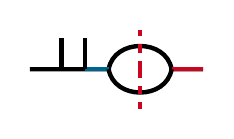
\begin{tikzpicture}
    \ver{e1}{-1,0};
    \ver{e2}{-0.6,0.4};
    \ver{e3}{-0.3,0.4};
    \ver{i1}{-0.6,0};
    \ver{i2}{-0.3,0};
    \ver{i3}{0,0};
    \ver{i4}{0.8,0};
    \ver{co}{$(i3)!0.5!(i4)$};
    \ver{e4}{1.2,0};
    \draw[ultra thick] (e1)--(i1)--(i2)--(i3) to [out=80,in=100,min distance=0.4cm](i4)--(e4);
    \draw[ultra thick](i1)--(i2);
    \draw[ultra thick,ucp-color](i2)--(i3);
    \draw[ultra thick,cut-color](i4)--(e4);
    \draw[ultra thick] (i3) to [out=-80,in=-100,min distance=0.4cm](i4);
    \draw[ultra thick] (e2) -- (i1);
    \draw[ultra thick] (e3)--(i2);
    \draw[ultra thick,dashed,cut-color] (co)--++(90:0.5);
    \draw[ultra thick,dashed,cut-color] (co)--++(-90:0.5);
  \end{tikzpicture}
  \right]
  \in   \begin{tikzpicture}
\begin{feynman}
\vertex (a1) at (-.8, -0.6) {1};
\vertex (a2) at (-.8, 0.6) {3};
\vertex (a3) at (-1, 0) {2};
\vertex [dot, scale=2](mid1) at (0,0){};
\vertex [dot, scale=1.5,hgrey0](mid2) at (0,0){};
\vertex [dot, scale=2](mid3) at (1,0){};
\vertex [dot, scale=1.5,hgrey0](mid4) at (1,0){};
\vertex (a4) at (1.8, 0) {4};
\diagram{
(mid1) --[ultra thick,](a1),
(mid1) --[ultra thick,](a2),
(mid1) --[ultra thick,](a3),
%(mid1) --[ultra thick,](mid3),
(mid1) --[ultra thick,out=60,in=120,min distance=0.4cm](mid3),
(mid1) --[ultra thick,out=-60,in=-120,min distance=0.4cm](mid3),
(mid3) --[ultra thick](a4),
};
\end{feynman}
\end{tikzpicture}
\end{equation}
in which one of the \textcolor{ucp-color}{uncut propagators} is set
equal to an \textcolor{cut-color}{external on-shell propagator}.
Discussions about how to resolve these types of singularities can be
found in Refs.~\cite{Minahan:1987ha, Bern:2012uf, 
  Geyer:2015bja,Geyer:2015jch,Edison:2020uzf, Edison:2022jln, Edison:2022smn}. In addition to the
bubble-on-external-leg cuts, there is a related class of cuts in which
an uncut propagator is set to zero by an \emph{internal cut
  condition}, for instance,
\begin{equation}
  \label{eq:other-path}
  \begin{tikzpicture}
    \pgfmathsetmacro{\ri}{1};
    \pgfmathsetmacro{\re}{0.6};
    \pgfmathsetmacro{\ang}{35};
    \begin{feynman}
      \blob{i1}{\ang:\ri};
      \blob{i2}{180-\ang:\ri};
      \blob{i3}{180+\ang:\ri};
      \blob{i4}{-\ang:\ri};
      \blob{i5}{ $(i1)!0.5!(i2)$ };
      \ver{e1}{45:\ri+\re};
      \ver{e2}{135:\ri+\re};
      \ver{e3}{225:\ri+\re};
      \ver{e4}{-45:\ri+\re};
      
      \diagram{
        {[edges={ultra thick}] (e1)--(i1),
          (e2)--(i2),
          (e3)--(i3),
          (e4)--(i4),
          (i5)--(i1)--(i4)--(i3)--(i2),
          (i2) --[out=60,in=180-60] (i5),
          (i2) --[out=-60,in=180+60] (i5)
        };
      };
    \end{feynman}
  \end{tikzpicture}
  \text{ contains a contribution from }
  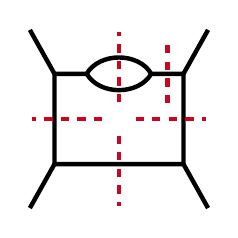
\begin{tikzpicture}
    \pgfmathsetmacro{\ri}{1};
    \pgfmathsetmacro{\re}{0.6};
    \pgfmathsetmacro{\ang}{35};
    \pgfmathsetmacro{\cang}{90};
    \pgfmathsetmacro{\cl}{1.1};
      \ver{i1}{\ang:\ri};
      \ver{i2}{180-\ang:\ri};
      \ver{i3}{180+\ang:\ri};
      \ver{i4}{-\ang:\ri};
      \ver{i5}{ $(i1)!0.25!(i2)$ };
      \ver{i6}{ $(i1)!0.75!(i2)$ };
      
      \ver{e1}{45:\ri+\re};
      \ver{e2}{135:\ri+\re};
      \ver{e3}{225:\ri+\re};
      \ver{e4}{-45:\ri+\re};

      \ver{c1}{0:\cl};
      \ver{c2}{\cang:\cl};
      \ver{c3}{2*\cang:\cl};
      \ver{c4}{3*\cang:\cl};
      \ver{ci}{$(i5)!0.5!(i1)$};
      \path let \p1 =(ci) in coordinate (c5) at (\x1,0.2){};
      \draw[ultra thick] (e1)--(i1);
      \draw[ultra thick] (e2)--(i2);
      \draw[ultra thick] (e3)--(i3);
      \draw[ultra thick] (e4)--(i4);
      \draw[ultra thick] (i5)--(i1)--(i4)--(i3)--(i2)--(i6);
      \draw[ultra thick] (i6) to[out=60,in=180-60] (i5);
      \draw[ultra thick] (i6) to[out=-60,in=180+60] (i5);
      \draw[dashed,ultra thick,cut-color] (0,0) -- (c1);
      \draw[dashed,ultra thick,cut-color] (0,0) -- (c2);
      \draw[dashed,ultra thick,cut-color] (0,0) -- (c3);
      \draw[dashed,ultra thick,cut-color] (0,0) -- (c4);
      \draw[dashed,ultra thick,cut-color] (c5) -- ++(90:0.7*\cl);
      \node[fill=white,circle] (c) at (0,0) {};
  \end{tikzpicture}.
\end{equation}
Fully resolving both of these problems is beyond the scope of the
current work, so we will simply not impose any constraints that
require handling these types of cuts.





\iffalse
The essence of generalized unitarity is that when internal lines are
placed on-shell, the integrand should factorize into a product of
on-shell tree amplitudes.  The cut to be performed can, itself, be
encoded in a graph.  For example, potential four-point two-loop cuts include
\begin{equation}
\label{eq:PotentialCuts}
\text{(a)} \SubtleCut ~~~~ \text{(b)} \PhysicalCutOne{}{}{}{} ~~~~ \text{(c)} \PhysicalCutTwo{}{}{}{} ~~~~ \text{(d)}  \MaxCut
\end{equation}
as well as many more.
In these graphs, all exposed propagators are understood to be cut/on-shell.
As an equation, a unitarity cut looks schematically like
\begin{equation}
\label{eq:SchematicCutEquation}
\sum \limits_\text{topologies} \frac{n \vert_\text{cut}}{\prod \limits_\text{uncut} k^2} = \sum \limits_\text{states} \prod \limits_\text{blobs} A_\text{tree} \, .
\end{equation}
The right hand side of the equation is a product of on-shell tree
amplitudes, represented graphically in \cref{eq:PotentialCuts} by grey
blobs.  States crossing (or propagating across) the cut must be summed
over.  For scalars this sum is trivial but for spinning particles this
is no longer the case and the physical state projector must be
inserted (see Dimitrius paper for simplifying this operation).  The
graph topologies appearing in the left hand side of
\cref{eq:SchematicCutEquation} come from blowing up the grey blobs
into cubic tree graphs in every conceivable way.  The numerator of
each graph is related back to the basis numerators via Jacobi
relations.  For each of these topologies, the numerator of the
associated graph is subjected to the cut constraints and is then
divided by the uncut propagators.  The right hand side is assumed to
be known, which places a constraint on the numerator ansatz in the
left hand side.

It is possible to work with either color-dressed cuts or color-ordered
cuts.  For color-dressed cuts the grey blobs are blown up into all
possible channels and all color factors $f^{abc}$ are explicitly
retained on both sides of the unitarity equation
\cref{eq:SchematicCutEquation}.  For color-ordered cuts the grey blobs
are only blown up in color-ordered channels, all color factors in
\cref{eq:SchematicCutEquation} are suppressed, and the product of
on-shell amplitudes only extends over color-ordered trees.  Since
color-ordered cuts do not contain the full color information of the
theory, it is necessary to do multiple color-ordered cuts -- over
different orderings of the blob labels -- in order to fully capture
all of the cut information.  For a color dual theory such as NLSM or
YM it is enough to do $(n-2)!$ labelings of each blob due to the
Kleiss-Kuijf and $U(1)$ decoupling identities (cite KK).  In this
sense color-dressed cuts contain extraneous information that is
bypassed when using color-ordered cuts.

In our construction, only well-defined cuts are imposed so, for
example, cut (a) of \cref{eq:PotentialCuts} is not enforced since it
is possible to blow up the left blob into a tree amplitude with an
on-shell internal propagator.  Cuts (b), (c), and (d) represent
physical cuts where (d) is known as a maximal cut since the maximal
number of propagators have been put on shell.  \fi

After imposing all four of the conditions above, any remaining free
parameters represent ``generalized gauge freedom'' meaning that the
freedom does not affect the physical integrand or its double copy.


\section{One-loop cubic construction}
\label{sec:cubic}
Here we will describe why constructing the full Yang-Mills kinematic
algebra (outside the self-dual sector) is generically hard, and why
the same reason makes NLSM beyond one-loop hard as well. The major
obstacle stems from the vector state sum mixing with higher-point
contacts. Starting with the Yang-Mills Lagrangian,
\begin{equation}
  \label{eq:ym-lag}
  \mathcal{L}^{\text{YM}} = -\frac{1}{2}(\partial_\mu A_\nu)^2
  + f^{abc} \partial_\mu A^a_\nu A^b_\mu A^c_\nu
  + f^{abe}f^{ecd}A^a_\mu A^b_\nu  A^c_\mu A^d_\nu 
\end{equation}
we can express the YM three-point interaction in terms of the
following vertex in Lorenz gauge:
\begin{equation}
\Acubic{hgrey0}{}{nhpRed}{}{nhpRed}{fermion2}{} =(\varepsilon_i\varepsilon_j)(\varepsilon_k p_i).
\end{equation}
This kinematic vertex is anti-symmetric in $1\leftrightarrow 2$
exchange, and from it we can construct the full Lorenz gauge
Yang-Mills vertex by summing over cyclic permutations,
\begin{equation}
V^{(123)}_{\text{YM}} = \Acubic{hgrey0}{}{nhpRed}{}{nhpRed}{fermion2}{}  +\text{cyc}(123)\,.
\end{equation}
Contracting this with the vector state sum, we can see that the cubic
Yang-Mills vertex does not satisfy the four-point Jacobi identity:
\begin{equation}
  \label{cubicJac}
  {}_1\langle V^{2}_{\text{YM}}V^{3}_{\text{YM}}\rangle_4+\text{cyc}(234) = \varepsilon_{(12)}  \varepsilon_{(34)} (s_{13}-s_{23}) +\text{cyc}(234) \neq 0
\end{equation}
where $ \varepsilon_{(ij)} = \varepsilon_{i}\cdot \varepsilon_{j}$.
However, the remaining terms can be absorbed into the definition of the
four-point kinematic numerator, as follows
\begin{equation}
{}_1\langle V^{2}_{\text{YM}+B}V^{3}_{\text{YM}+B}\rangle_4 = {}_1\langle V^{2}_{\text{YM}}V^{3}_{\text{YM}}\rangle_4 + s_{12} (\varepsilon_{(13)}\varepsilon_{(24)}-\varepsilon_{(14)}\varepsilon_{(23)})
\end{equation}
Note that this new definition of the $s$-channel numerator contains two factors of $\varepsilon_{(ij)} $ that contract spacetime indices \textit{across} the factorization, suggesting the inclusion of a spin-2 mode. As such, we use $V_{\text{YM}+B}$ to denote the inclusion of an additional two-form, as was studied in Ref.~\cite{Ben-Shahar:2022ixa} for constructing the NMHV Yang-Mills Lagrangian.  After the introduction of the two-form, the
numerators now satisfy the Jacobi identity:
\begin{equation}
  {}_1\langle
  V^{2}_{\text{YM}+B}V^{3}_{\text{YM}+B}\rangle_4+\text{cyc}(234) =0\,,
\end{equation}
where the new cubic Lagrangian takes the form\,,
\begin{equation}
\mathcal{L}^{\text{YM}+B} = -\frac{1}{2}(\partial_\mu A_\nu)^2 -
B_{\mu\nu}\Box\tilde{B}_{\mu\nu}+ f^{abc} \partial_\mu A^a_\nu A^b_\mu
A^c_\nu+ f^{abc} (B_{\mu\nu}+\Box \tilde{B}_{\mu\nu})^a A^b_\mu
A^c_\nu\, .
\end{equation}
Of course, higher multiplicity would likely require further redefinition of
the three-point vertex to satisfy Jacobi identities on all internal
edges. While introducing successively higher spin states could in
principle work at tree level, we will see that it is not consistent
with what we find at general loop order. We will comment on this in
\cref{sec:Discussion} \ace{Is this the sec you are thinking of?} \nhp{ Yes. thanks :-)}. For
now, we will study how to construct one-loop integrands consistent
with the color-kinematics by isolating the cubic sector of the state
sum above.

As can be seen above, the Jacobi identity of \cref{cubicJac} fails
only in terms with two factors of polarization dot products,
$(\varepsilon\varepsilon)^2$. Whereas if we restricted ourselves to
just considering factors with a single polarization dot product, the
Jacobi identity of Yang-Mills would be satisfied \textit{off-shell}
and in arbitrary spacetime dimensions
\begin{equation}
{}_1\langle V^{2}_{\text{YM}}V^{3}_{\text{YM}}\rangle_4\big|^{(\varepsilon\varepsilon)^1}+\text{cyc}(234) =0\,.
\end{equation}
\ace{Should we mention that this is closely related to MHV vs NMHV?} \nhp{Yes, I added a couple sentences and reference below -- let me know what you think}.

This restriction to the $(\varepsilon\varepsilon)^1$ cubic sector of Yang-Mills is closely related to the MHV decomposition of color-dual numerators \cite{ElvangHuangReview,Chen:2019ywi,Chen:2021chy}, where choosing appropriate reference vectors sends all $(\varepsilon\varepsilon) \rightarrow 0$, with the exception of one of the positive helicity polarizations, $\varepsilon^+_1$, dotted into all the $n-2$ negative helicity modes in the full MHV amplitude, $\varepsilon^+_1 \varepsilon^-_i \neq 0$. We describe this in detail in \cref{Conventions}. With the interest in constructing dimension agnostic color-dual integrands at one-loop, we want to avoid making specific reference to 4D helicity states.

Thus for our approach at one-loop, we aim to build color-dual integrands directly from $D$-dimensional kinematic factors that are $\mathcal{O}((\varepsilon\varepsilon)^1)$ at tree-level, and $\mathcal{O}((\varepsilon\varepsilon)^0)$ at one-loop. The $D$-dimensional organizational principle underlying this construction can be understood in terms of a vector amplitude decomposition introduced by one of the authors \cite{Pavao:2022kog},
\begin{equation}\label{eq:pureVecRABD}
A_{(\sigma)}^{\text{YM}} = \sum_{k=0}^{\lfloor |\sigma|/2\rfloor}\sum_{\rho \in S^{2|k}_{\sigma}}\varepsilon_{(\rho)} \Delta_{(\sigma)}^{(\rho)}\,.
\end{equation}
where we have introduced the shorthand notation, $\varepsilon_{(ij)\cdots (kl)} \equiv (\varepsilon_i \varepsilon_j)\cdots (\varepsilon_k \varepsilon_l)$, and  $S^{2|k}_{\sigma}$ is the set of $k$ pairs of external legs appearing in the color-ordered label list, $\sigma$. For example, at four-point, $S^{2|1}_{\sigma} =  \{(12),(13),(14),(23),(24),(34)\}$, and $S^{2|2}_{\sigma} =  \{(12)(34),(13)(24),(14)(23)\}$. The sum thus selects out kinematic building blocks, $\Delta_{(\sigma)}^{(\rho)}$,that are each weighted by different polarization dot products. Some simple four-point examples include, 
\be
\Delta^{(13)}_{(1234)} =\frac{(k_1 \varepsilon_2)(k_{3} \varepsilon_4)}{s_{12}}+\frac{(k_1 \varepsilon_4)(k_{3} \varepsilon_2)}{s_{14}}, \qquad \Delta^{(13)(24)}_{(1234)} =1, \qquad \Delta^{(12)(34)}_{(1234)} =\frac{s_{13}}{s_{12}}\,. 
\ee
We direct the reader to ref.~\cite{Pavao:2022kog} for further details. By a simple mass-dimension argument \cite{ElvangHuangReview}, we know the tree-level cubic sector of Yang-Mills must be at
$\mathcal{O}((\varepsilon\varepsilon)^1)$,
\begin{equation}
A_{(\text{tree})}^{\text{cubic-YM}} = \sum_{\rho \in S^{2|1}_{\sigma}}\varepsilon_{(\rho)} \Delta_{(\sigma)}^{(\rho)}\, ,
\end{equation}
while at one-loop, the cubic sector corresponds to
$\mathcal{O}((\varepsilon\varepsilon)^0)$ in polarization dot
products,
\begin{equation}
A_{(\text{1-loop})}^{\text{cubic-YM}} = \sum_{\rho \in S^{2|0}_{\sigma}}\varepsilon_{(\rho)} \Delta_{(\sigma)}^{(\rho)}\,.
\end{equation}
When decomposed in this way, the polarization stripped building blocks
must obey a set of Ward-identities between different ``helicity'', or
$(\varepsilon \varepsilon)^n$, sectors in order for the full amplitude
to be gauge invariant,
 \begin{equation}\label{eq:GIrelA}
\Delta_{(\sigma)}^{(\rho)}\Big|_{\epsilon_i\rightarrow k_i} =-
\sum_{j \in \rho^c} (k_i \varepsilon_j)\Delta_{(\sigma )}^{(\rho\cup (ij))} \,.
\end{equation}
With this in hand, we can construct a Lagrangian description of the of
the cubic sector for Yang-Mills, and will demonstrate that the
resulting amplitudes with manifestly color-dual Feynman rules are
equivalent to both SDYM and NLSM through one-loop.


\subsection{Semi-abelian Yang-Mills theory}\label{semiYM}
As we argued above, if we include factors of
$(\varepsilon\varepsilon)^{n\geq 1}$ at tree-level, then we need to
keep the Yang-Mills four-point contact for color-kinematics duality to
be restored on-shell. However, the contrapositive is also true -- if
we omit the four-point Yang-Mills vertex, then we only need terms that
contribute to the manifestly color-dual cubic sector of the theory.

We can achieve this construction by splitting the gauge group of the
full Yang-Mills action from $G$ to $G_L \times G_R$, where the full
non-abelian gauge symmetry is restored only when we identify
$G_L = G_R$. However, if we break the left gauge group down to
$G_L \rightarrow U(1)^{N^2}$ and take the right gauge group to
$G_R \rightarrow U(N)$, then we are left with a semi-abelian theory
that is gauge invariant in the preferred $U(1)$-directions. We call
this manifestly color-dual theory \textit{semi-abelian Yang-Mills},
\begin{eBox}
\begin{equation}
\label{eq:semiYM}
\mathcal{L}^{\text{semi-YM}} = -\frac{1}{2}\text{tr}\left[\bar{F}_{\mu\nu}F^{\mu\nu}\right]
\end{equation}
\end{eBox}
where
\begin{equation}
\bar{F}^a_{\mu\nu} = \partial_\mu \bar{A}_\nu^a - \partial_\nu \bar{A}_\mu^a
\end{equation}
\begin{equation}
F^a_{\mu\nu} = \partial_\mu A_\nu^a - \partial_\nu A_\mu^a + f^{abc} A_\mu^b A_\nu^c
\end{equation}
and $A_\mu$ is in Lorenz gauge.
Here we can think of the abelian vector as a background field that
sources on-shell $A_\mu$ currents. Indeed, as we describe in Appendix
\cref{sec:CKLagrangians}, semi-abelian Yang-Mills theory is at the
heart of YZ-theory \cite{Cheung:2016prv}, J-theory
\cite{Cheung:2020djz,Cheung:2021zvb}, and self-dual Yang-Mills
\cite{Monteiro2011pc}.  Specifically, semi-Abelian YM is simply a
clever reinterpretation of the Lagrangian obtained by integrating an
auxiliary field into the J-theory equations of motion.  The Feynman
rule for the cubic vertex is
\begin{equation}
  \cubic{hgrey0}{fermion2}{}{fermion2}{}{fermion2}{}= (\varepsilon_1\bar{\varepsilon}_3)(\varepsilon_2 k_3)
  -  (\varepsilon_2\bar{\varepsilon}_3)(\varepsilon_1 k_3).
\end{equation}
where the incoming arrow is the abelianized gauge field, and the outgoing arrows the on-shell non-abelian vectors. The propagator is simply:
\be
\propFrule{$A^\nu$}{$\bar{A}^\mu$}{$k \rightarrow $}{fermion2} = \frac{i}{k^2} \eta^{\mu\nu}
\ee
As one can see, the kinetic term mixes the two gauge fields and has the standard
Feynman rule of $i/k^2$.  We can use the Ward identity of
\cref{eq:GIrelA} to check that the amplitudes are indeed gauge
invariant when the abelian polarizations are taken to be longitudinal,
$\bar{\varepsilon} \rightarrow k$.

As noted above, we can select out can manifestly cubic
sector of semi-abelian Yang-Mills from the full theory of \cref{eq:ym-lag} by selecting only $(\varepsilon^+\varepsilon^+)$ in light-cone gauge (i.e. SDYM) and one-minus at tree-level or by plugging in the on-shell states of $J$-theory \cite{Cheung:2020djz,Cheung:2021zvb} and
$YZ$-theory \cite{Cheung:2016prv}. Indeed, the
$D$-dimensional description of $J$-theory is just the following blocks
in the expansion of Yang-Mills given in Ref.~\cite{Pavao:2022kog}
\begin{equation}
A(...,\bar{A}_k,...)_{\text{tree}} = \sum_{j\neq k}\Delta^{(jk)}_{\text{tree}}
\end{equation}
and similarly so at one-loop
\begin{equation}
A(...)_{\text{1-loop}} \equiv \Delta^{(\varnothing)}_{\text{1-loop}}\, .
\end{equation}
To recover NLSM at one-loop, we need to extract the $D$-dependent part
that corresponds to an internal $\bar{Y}Y$-loop from extra-dimensional
scalars
\begin{eBox}
\begin{equation}
A^{\text{NLSM}}_{\text{1-loop}} \equiv \partial_D \Delta^{(\varnothing)}_{\text{1-loop}}\big|_{\varepsilon\rightarrow k}\, .
\end{equation}
\end{eBox}
Why must we take the derivative with respect to $D$? After all,
$J$-theory and $YZ$-theory both have well defined propagators for
internal $\bar{J}J$ and $\bar{Z}Z$ propagators. However, as we discuss
in \cref{sec:CKLagrangians}, all the $J$ and $Z$ states must be on-shell in order to
produce NLSM amplitudes. Thus, the unitarity cuts of $J$ theory at
one-loop will not produce NLSM amplitudes. However, the internal
$YY$-loop is a valid forward limit for producing NLSM amplitudes,
since as constructed YZ theory matches to NLSM for off-shell
Y-particles. We provide explicit expressions for these one-loop amplitudes in the next section.

\subsection{One-loop color-dual integrands}\label{oneLoopCK}
Our first application of this theory for color-dual construction at
loop level is for self-dual Yang-Mills (SDYM). At tree-level, the
off-shell cubic vertices can be written in terms of light cone
coordinates \cite{Monteiro2011pc}:
\begin{equation}
X(p,k) = p_u k_w-p_w k_u
\end{equation}
At loop-level, this construction needs to be analytically continued to
general dimension in order to apply dimensional regularization at
one-loop. This can be done using the cubic semi-YM vertices of the
previous section:
\begin{equation} \label{DdimSDYM}
\cubic{hgrey0}{fermion2}{}{fermion2}{}{fermion2}{}= \mathcal{X}(k_1,k_2) = (\varepsilon_1\bar{\varepsilon}_3)(\varepsilon_2 k_3) -  (\varepsilon_2\bar{\varepsilon}_3)(\varepsilon_1 k_3)
\end{equation}
Plugging in on-shell all-plus helicity states in light-cone gauge will
yield precisely the 4D SDYM vertex, up to an unphysical phase \ace{Can
  we provide an example?} \nhp{yes, provided}:
  \be
  \mathcal{X}(k^+_1,k^+_2) = \frac{\langle 12\rangle^3}{ \langle23\rangle \langle 31\rangle} \sim \langle 12\rangle = k_{1,u} k_{2,w}-k_{1,w} k_{2,u}
 \ee
where $\mathcal{X}(k^+_1,k^+_2) = A^{\text{YM}}(1^+,2^+,3^-)$ in light cone gauge, and in the second step applied momentum conservation to redefinition of the spinor bracket, $\langle 12\rangle \rightarrow X(p,k)$ defined in \cref{Conventions}. Of course, the form of \cref{DdimSDYM} has the advantage of
permitting a $D$-dimensional construction of the one-loop
integrand. Below we provide a four-point example:
\begin{equation}
\simplebox = g_{\text{YM}}^4 \langle \mathcal{X}(k_1,l_1)\mathcal{X}(k_2,l_2)\mathcal{X}(k_3,l_3)\mathcal{X}(k_4,l_4)\rangle
\end{equation}
where $l_i = l+k_1+k_2+\cdots+ k_i$ and the bracket $\langle \cdots\rangle$ indicates that we have applied the off-shell state projector, $\sum {\varepsilon^\mu_{(+l_i)}\varepsilon^\nu_{(-l_i)}}=P_{(l_i)}^{\mu\nu}$ on all internal polarizations. In general, the $n$-gon vertex would be
\begin{equation}
\mathcal{N}^{\text{SDYM}}_{n\text{-gon}}= \nGonVector = g_{\text{YM}}^n \langle \mathcal{X}(k_1,l_1)\mathcal{X}(k_2,l_2)\cdots \mathcal{X}(k_n,l_n) \rangle
\end{equation}
Due to the state-sum of internal loop factors,
$\sum {\varepsilon_{(+l)}\varepsilon_{(-l)}}\sim D$, the integrand above
depends explicitly on the spacetime dimension, $D$. By taking a
derivative\footnote{Another way to understand this derivative is that
  it selects the large $D$ behavior of the integrand.}, we can recover
the integrand needed for all-plus one-loop amplitudes with an internal
scalar:
\begin{equation}
\partial_D \mathcal{N}^{\text{SDYM}}_{n\text{-gon}}=\nGonScalar  = (2 g_{\text{YM}})^n (l_1 \varepsilon_1)(l_2 \varepsilon_2)\cdots (l_n \varepsilon_n)
\end{equation}
This integrand numerator with internal scalar loop is precisely what
one would obtain from the Feynman rules of YZ-theory, absent the $\bar{Z}Z$
internal vector loop. For more background, we refer the reader to
\cref{sec:CKLagrangians}. When plugging on the on-shell states of $YZ$-theory, we thus obtain the following expression for the NLSM one-loop $n$-gon numerator:
\begin{equation}
 \mathcal{N}^{\text{NLSM}}_{n\text{-gon}}=\left[\partial_D  \mathcal{N}^{\text{SDYM}}_{n\text{-gon}}\right]^{\epsilon \rightarrow k}=\nGonScalar =  f_\pi^{-n} [12][23]\cdots [n1]
\end{equation}
Where we have define the antisymmetric kinematic variable, $[LR] = l_L^2 - l_R^2$, since when plugging on longitudinal modes, the $n$-gon can be re-expressed completely in terms of inverse propagators, $2(k_i \cdot l_i) = l_{i}^2-l^2_{i-1}$. We have verified through 10-point one-loop that this $n$-gon expression is a valid color-dual representation for NLSM. 

Before proceeding, we note that the above definition does give rise to ``pathological" bubble-on-external-leg (BEL) diagrams discussed previously in \cref{sec:bootstrap}. However, one can show that these diagrams integrate to zero for spacetime dimension, $D>2$, and thus can be disregarded as unphysical. For the interested reader, in \cref{BELreg} we provide a detailed overview of this dimensional regularization of the BEL diagram.
\subsection{Two-loop obstruction}\label{2LoopObstruction}
At two-loop, introducing terms that conspire with four-point contacts
is unavoidable. At one-loop, we were able to avoid internal
contractions of $\bar{A}_\mu A^\mu$ by selecting appropriate external
states. However, at two-loop when choosing all external $A_\mu$
states, the amplitude vanishes in semi-YM theory:
\begin{equation}
\mathcal{A}^{\text{semi-YM}}_{\text{2-loop}}(A_\mu,A_\mu,A_\mu,A_\mu)=0
\end{equation}
In order to produce non-vanishing interactions, we would need to
reintroduce $D$-dimensional vertices from the diagonal group of
$G_L\times G_R$ that have the wrong weight. Doing so will necessarily permit internal
contractions of $\bar{A}_\mu A^\mu$,
\begin{equation}
\mathcal{A}^{\text{YM}}_{\text{2-loop}}(A_\mu,A_\mu,A_\mu,A_\mu)=\doubleBoxObstructionA +\doubleBoxObstructionB+\cdots 
\end{equation}
where we used white dots to indicate interaction vertices of weight\footnote{We choose the convention that the abelianized gauge fields carry weight $\mathcal{W}[\bar{A}] = -1$, and non-abelian vectors are $\mathcal{W}[\bar{A}] = +1$.} $\mathcal{W}[\bar{A}\bar{A} A] = -1$, rather than the isolated semi-YM vertex which always carries weight $\mathcal{W}[\bar{A}A A] = +1$. This immediately runs into the difficulty of introducing the
four-point contact needed for color-kinematics to be satisfied on all
internal edges. By a simple weight counting argument, one can see that including this wrong sign interactions is unavoidable at two-loop and higher. 

Thus, to construct two-loop numerators prescriptively, as we have done at one-loop, would require knowledge of
the full kinematic algebra for Yang-Mills off-shell. Since this is
presently unavailable, to approach the problem of two-loop
construction, we instead employ an ansatz based approach.


\section{Two-loop bootstrap}
\label{2loopBoot}
\ace{Lets bulk this section intro up a bit} \nhp{Is this sufficient?}

We now employ the color-dual bootstrap method described in
\cref{sec:bootstrap}. We will start with an ansatz constructed from
$D$-dimensionally Lorentz covariant kinematics. To fix remaining
freedom in the NLSM bootstrap, we will match down to ZM theory in
$D=2$. This is merely an aesthetic choice, so the final results of
both the NLSM and Yang-Mills bootstraps are dimensionally agnostic.


\subsection{Two-loop NLSM}
\label{sec:pions}

As we have seen, it is possible to coerce tree numerators into 1-loop
numerators at any multiplicity for pions.  However, these methods
cannot be reapplied to generate higher-loop numerators, which begs the
question ``is it possible to find globally color-dual numerators
beyond 1-loop?''  We will tackle this question for four-point two-loop
scattering in NLSM before moving on to the same process in YM.

Ignoring tadpoles and BEL graphs, there are 14 cubic four-point two-loop
graphs (see \cref{fig:MaxCuts}) which are related to each other via 21
Jacobi relations.  As mentioned in \cref{sec:bootstrap},
color-kinematics duality ensures that the numerator of every graph can
be expressed in terms of a basis of the double box and penta-triangle,
\begin{equation}
\label{eq:jacobi-basis}
\NLSMBasisDoubleBox \text{ and } \NLSMBasisPentaTriangle .
\end{equation}
For a scalar theory like NLSM the numerator only depends on dot
products of momenta.  The basis of momentum invariants for both of
these graphs can be taken to be
\begin{equation}
\label{eq:scalar-basis}
\{ k_{13}, k_{23}, k_{15}, k_{16}, k_{25}, k_{26}, k_{35}, k_{36}, k_{55}, k_{56}, k_{66} \},
\end{equation}
where $k_{ij}$ means $k_i \cdot k_j$, $k_5=\ell_1$, and $k_6 = \ell_2$.
%%%%
% Basis for both diagrams
% {d[p[1], p[3]], d[p[1], p[6]], d[p[1], p[7]], d[p[2], p[3]],  d[p[2], p[6]], d[p[2], p[7]], d[p[3], p[6]], d[p[3], p[7]],  d[p[6], p[6]], d[p[6], p[7]], d[p[7], p[7]]}
%%%%
Every vertex in NLSM scales as $k^2$ so the numerator of each diagram
scales as $k^{12}$.  At this mass dimension there are 8,008
independent dot products of momenta.  With two basis graphs there is a
total of 16,016 ansatz parameters.\footnote{\texttt{Mathematica} is
  not suited to equations with sixteen thousand parameters so a
  different method is desirable.  One possibility is to use a solver
  designed for integral reduction.  However, these solvers typically
  assume that the matrix has a very low density which is not the case
  for equations coming from NLSM which typically have a density of a
  few percent.  While the equations in YM naturally separate into
  different ``helicity'' sectors (or $e_i \cdot e_j$ and
  $e_i \cdot k_j$ sectors in $D$ dimensions), there is no such
  separation of sectors in a scalar theory where any product of
  momenta can interfere with any other.  The NLSM constraint equations
  were solved using a custom solver, \texttt{FiniteFieldSolve},
  designed to solve large linear systems of arbitrary density.
  \texttt{FiniteFieldSolve} will be released publicly shortly.\ace{I
    want to rephrase this slightly, but need to think about it a bit
    more}} Imposing the boundary Jacobi relations eliminates all but
4,473 of the original free parameters.  Further imposing graph
symmetries reduces the number of free parameters to 1,243.

\begin{figure}
  \begin{center}
	\PhysicalCutOne{}{}{}{} \PhysicalCutTwo{}{}{}{}
  \end{center}
  \caption{The two physical cut topologies shared by NLSM, sGal, BI, and DBIVA}
  \label{fig:emu}
\end{figure}

The final essential constraint is unitarity.  The two physical cuts
that need to be enforced, shown in \cref{fig:emu}, only involve
four-point vertices.  Notably this means that even at two loops,
unitarity is still only probing the on-shell four-point NLSM amplitude.
Unitarity cuts besides those shown in \cref{fig:emu} are either
pathological or vanish because they involve a 3pt point on-shell
amplitude (which vanishes on general grounds for scalar theories
\ace{This feels like overstating things.  For instance, what about
  $\phi^3$ or BAS?}).  In order to manifest the $\mathbb{Z}_2$
symmetry of NLSM at the integrand level, we require that all
non-pathological cuts containing a 3pt vertex (such as the maximal
cut) vanishs.  Imposing all relevant cuts leaves 765 free parameters
representing the generalized gauge freedom in the answer.

% It is possible to automatically enforce (or ``bake in'') the double
% box and penta-triangle max cuts on the ansatz by writing the ansatz
% in terms of inverse propagators (and remaining irreducible scalar
% products) and then only keeping terms that involve at least one
% inverse propagator since those terms will vanish on those max cuts,
% just as the product of 3pt scalar amplitudes will.  However, for the
% sake of simplicity we do not take this route.

At this point color-kinematics duality has been satisfied, so the
double copy will proceed without issue.  However, the plethora of
generalized gauge freedom parameters leaves the option for enforcing
additional aesthetic constraints.  All remaining generalized gauge
parameters could be set to zero, but a simpler and more insightful
result can be obtained through physical arguments.  $\mathcal{N}=4$
SYM provides several hints for further conditions to impose on the
ansatz.  For example, for maximally supersymmetric gauge theory it is
possible to enforce the no triangle hypothesis, manifest loop power
counting, and, for four-point and up to at least six loops, strip off a
factor of $st \atree$ from the integrand \cite{FiveLoopN4,
  Bern:2012uf, Bern:2010fy, SuperSum, Carrasco:2021otn,
  JJHenrikReview, BRY, BDDPR, Neq44np}.  For the NLSM integrand it is
desirable to make color-kinematics duality as manifest as possible.
One hope would be to factor out some piece of the one-loop numerator
since this at least manifests antisymmetry for the vertices involving
external legs.  However, a more fruitful direction is to match onto
the one known theory with pion power counting that manifests
color-kinematics duality to all loop orders, namely,
Zakharov-Mikhailov (ZM) theory \cite{Zakharov:1973pp, Cheung:2022mix}. ZM theory is governed by the Lagrangian
\begin{equation}
\label{eq:ZMLagrangian}
\mathcal{L}^{\text{ZM}} = \frac{1}{2}(\partial \varphi)^2
+ g f^{abc} \varphi^a \varepsilon^{\mu\nu}(\partial_\mu \varphi^b)( \partial_\nu \varphi^c),
\end{equation}
where more details can be found in \cref{sec:CKLagrangians}.  The
color-stripped Feynman rule for the vertex is
$V(k_1, k_2, k_3) \propto \varepsilon_{\mu\nu}k_1^\mu k_2^\nu$ where
off-shell color-kinematics duality to all orders in perturbation
theory simply follows from the Schouten identity in 2D.  Since the theory
only has a cubic vertex and manifest off-shell color-kinematics
duality, it is trivial to read off the color-dual numerator for any
graph.  From the presence of the Levi-Civita tensor
$\varepsilon^{\mu\nu}$, the theory clearly resides in two spacetime
dimensions where scattering is notoriously plagued by infrared
regulation issues.  Every on-shell particle is either a right mover,
with momentum proportional to $k_R^\mu \equiv (1,1)$, or a left mover,
with momentum proportional to $k_L^\mu \equiv (1,-1)$.  On-shell ZM
amplitudes naturally divide into sectors corresponding to the
configuration of left and right movers, where the scattering in many
sectors is rather subtle.  Only color-ordered amplitudes can be
defined unambiguously from the Feynman rules.  At four-point, only the
alternating sector is free of subtleties and the amplitude for this
process vanishes.  In equations, $A[LRLR]=0$ where $R$ corresponds to
a right mover and $L$ corresponds to a left mover.  In every other
configuration of right and left movers, such as $A[RRRR]$, one of the
internal propagators is accidentally on-shell since $k_R^2=k_L^2=0$.

\ace{Lets tighten up this paragraph a bit, especially the second half}
It is tempting to try to match the pion four-point two-loop integrand to ZM
on the cuts, but given that the cuts only probe the on-shell four-point
amplitude, which is either subtle or vanishes for ZM, it is better to
compare the off-shell numerators directly.  As local functions, the
numerators never suffer from any of the subtleties of on-shell 2D
kinematics.  Since the physical cuts are difficult to compare, ZM
theory is being used here simply as a tool to eliminate generalized
gauge freedom; ZM theory has the right power counting and kinematic
structure in 2D to compare against.  Since ZM theory is only being
used for the kinematical structure of its numerators, it is natural to
introduce a proportionality constant $z$ between the NLSM and ZM
numerators $n_\text{NLSM} \vert_{2D} = z ~ n_\text{ZM}$.  The
parameter $z$, which would normally be fixed on cuts, effectively
encodes the discrepancy between the coupling constants of the two
theories.\footnote{Floating the proportionality parameter $z$ is also
  motivated because ZM is believed to be quantum mechanically
  different from NLSM even though they are dual classically in two
  dimensions \cite{Nappi:1979ig}.}  This introduces an extra degree of
freedom into the problem.  Mechanically, the pion numerator is matched
to ZM by first taking every possible assignment of right and left
movers for the external particles and then restricting the pion
numerator to 2D.  The loop momenta are restricted to 2D but left
off-shell.  After performing the 2D matching, there are only 365
parameters of generalized gauge freedom.

The loop momentum structure of ZM theory provides one final hint for
simplifying the pion numerators.  A generic term in the ZM numerator
(of either basis graph) looks schematically like
\begin{equation}
\label{eq:ZMLoopPowCount}
\ell_1^m \ell_2^n k^{12-(m+n)} \text{ where } 5 \leq m+n \leq 8,
\end{equation}
whereas a generic set of local, cubic Feynman rules could have
produced terms with up to $m+n=12$ powers of loop momenta.  When the
pion numerator is forced to have the loop power counting structure in
\cref{eq:ZMLoopPowCount} of ZM theory, the number of generalized gauge
freedom parameters reduces to 58.  The pion numerator appearing in the
ancillary files makes exactly this choice.\footnote{When the four-point
  pion amplitude is normalized to $-k_1\cdot k_2$ and the ZM vertex is
  normalized to $k_1^\mu \varepsilon_{\mu\nu}k_2^\nu$, the parameter
  $z$ is fixed to $216/565$, which is clearly unrelated to the
  difference in coupling constants.} \ace{Is this actually where we
  want this particular footnote to appear?}

\subsection{Double-copy verification}
\label{doubleCopyVerify}

With a cubic color-dual pion representation in hand, we can perform
double copies with many theories to extract colorless gravity-like
amplitudes.  In particular, we produce numerators for special
Gallileons, Born-Infeld theory, and DBIVA by double-copying against
pions, $\mathcal{N}=0$ YM, and $\mathcal{N}=4$ sYM respectively
\cite{Cachazo:2014xea,Cheung:2015ota,Cheung:2016drk}.  Such double-copy constructions are important nontrivial
checks on the underlying single-copy theories as the Jacobi relations
in the single copy conspire to produce the double-copy theory's
version of linear diffeomorphism invariance: enhanced shift symmetry for special Galilleons, and gauge
invariance of the BI photon and DBIVA supermultiplet \cite{Hinterbichler:2015pqa}.  All
three of these double-copy theories were recently studied extensively
by one of the authors and Carrasco from the perspective of direct
unitarity cut construction \cite{Carrasco:2023qgz}.  One of the shared
features of these three theories is that they all have the same
physical cut topologies in 4D: the two diagrams shown in
\cref{fig:emu}, which are only composed of four-point amplitudes.

To construct the double-copy theories, we source the cubic
$\mathcal{N}=0$ YM numerators from Ref.~\cite{Bern:2015ooa} (which
additionally satisfies a relaxed form of color-kinematics duality),
and the cubic $\mathcal{N}=4$ sYM representation from the well-known
$n_{2\text{box}} = n_{\text{cross-box}} = s^2t\, \atree$ \cite{Bern:1997nh}.
On the other hand, we use the methods of Ref.~\cite{Carrasco:2023qgz}
to directly compute the needed basis cuts in all three theories without
relying on a color-dual pion representation.  We find exact agreement
in each of the three theories for both physical cuts.  Since
Ref.~\cite{Carrasco:2023qgz} has already exhaustively explored the
properties of four-point loop amplitudes in these theories, we direct
interested readers there for more information.


\subsection{Two-loop Yang-Mills revisited}\label{2loopYM}

\jm{Rather than quoting the number of parameters in the BDN ansatz, I
  would prefer to just focus on what we did since it's more general.
  I don't want it to sound like we just patched a minor hole in their
  argument when I think you've done something much cooler by
  pinpointing the failure to the bowtie graph. I know you put time and
  effort into analyzing the BDN ansatz but I'm worried that the more
  we talk about it, the more it will overshadow the real success
  here.}

Given the close ties between pion and gluon scattering for trees and
at one loop, the existence of the two-loop pion numerator prompts us
to investigate the most general local numerator for YM, without any of
the loop power counting assumptions of Ref.~\cite{Bern:2015ooa}.  We
follow the same general procedure as in \cref{sec:pions}, again
identifying the double-box (2box) and penta-triangle (pt) as the
Jacobi basis graphs and building a the most general ansatz for each of
their numerators compatible with the assumptions in
\cref{sec:bootstrap}.  Because we are now considering pure
Yang-Mills, each monomial in the local ansatz must consist of five
Lorentz scalar dot product s instead of the six for NLSM, and each
monomial must be linear in each of the four external gluon
polarizations.  Thus, the numerator ansatz for both diagrams will be
built from terms of the form:
\begin{equation}
  \mathcal{N}^{\text{YM}}\left[\NLSMBasisDoubleBox \right]\text{ and }\mathcal{N}^{\text{YM}}\left[\NLSMBasisPentaTriangle \right]\in \text{span}\left\{(\varepsilon_i \varepsilon_j) , (k_i \varepsilon_j), (k_ik_j)\right\}
  \label{eq:ym-basis}
\end{equation}
where the $k_i$ take the same definition as described near
\cref{eq:scalar-basis}.  In our labeling of the two loop Jacobi-basis
diagrams, shown in \cref{eq:jacobi-basis}, we find that the power
counting bound proposed by Bern, Davies, and Nohle leads to an initial
ansatz with 10,000 terms in the double-box, and 9849 terms for the
penta-triangle.  Without power counting restrictions, both the
double-box and the penta-triangle ansatz have an ansatz with 10,010
terms each.  Imposing diagram automorphisms and maximal-cut gauge
invariance on the two basis diagrams, we reduce the number of terms to
XX for the double-box, and YY for the penta-triangle.  In
Ref.~\cite{Bern:2015ooa}, the unitarity matching constraints were
imposed using a spanning set of minimal physical cuts, shown in
\cref{fig:ym-spanning}.  Instead of also directly going to the
spanning cuts, we work within the framework of the Method of Maximal
Cuts \cite{Bern:2007ct} in order to identify the simplest cut that is in
tension with the kinematic Jacobi relations.

\begin{figure}
  \begin{center}
    \begin{subfigure}{0.3\textwidth}
      \begin{center}
        \LMCut
      \end{center}
    \end{subfigure}
    \begin{subfigure}{0.3\textwidth}
      \begin{center}
        \PhysicalCutOne{}{}{}{}
      \end{center}
    \end{subfigure}
    \begin{subfigure}{0.3\textwidth}
      \begin{center}
        \PhysicalCutTwo{}{}{}{}
      \end{center}
    \end{subfigure}
  \end{center}
  \caption{The three spanning physical unitarity cuts of pure
    Yang-Mills at 2 loops}
  \label{fig:ym-spanning}
\end{figure}

Similar to the pion construction in \cref{sec:pions}, we use the
kinematic Jacobi relations to define the numerators for all cubic
graphs in terms of the two basis graphs, including allowing nontrivial
numerators on BEL diagrams.  We will simply avoid imposing constraints
that directly involve such pathological diagrams.  That again leaves
us with the 14 non-pathological cubic diagrams shown above in
\cref{fig:MaxCuts}, on which to impose maximal cuts and symmetries.
Doing so, we are left with AA total parameters in the unrestricted
ansatz.



Proceeding to the next-to-maximal cuts, we continue to avoid
pathological diagrams including the newly-appearing type discussed in
\cref{eq:other-path}.  After discarding these types of cuts as well as
those involving cuts of external Mandelstams, there are 8 cut
topologies (see \cref{fig:ym-nmc}).  Seven of these next-to-maximal
cuts are consistent with the kinematic Jacobi relations and
symmetries.  Critically, the ``bowtie'' cut,
\begin{equation*}
   \NMCutC \,,
\end{equation*}
cannot be satisfied by either the ansatz with Jacobi relations and
symmetries applied.

\begin{figure}
\centering
 { \NMCutH, \NMCutG,  \NMCutD,\NMCutB, 
 \\
 \NMCutE, \NMCutF, \NMCutA, \NMCutC,  }
  \caption{The 8 non-pathological 1-particle-irreducible next-to-maximal-cut diagrams used in our cut constraints on the Yang-Mills integrand.}
  \label{fig:ym-nmc}
\end{figure}

In fact, we can make the failure extremely precise.  Start with the
diagrams shown in the Jacobi relation from \cref{eq:TwoLoopJacobiOne}:
the double-box, crossed-box, and penta-triangle.  For each of the
three diagrams, write down the most generic parity-even local ansatz
involving four polarizations and six momenta (any combination of
external or loop).  Each ansatz will have 10,010 terms initially.  Next
impose the symmetry constraints on each of the three diagrams, leaving
2761 free parameters on the double-box, 2576 free parameters on the
crossed-box, and 5040 free paramters on the penta-triangle.  Then
impose the ``bowtie'' next-to-maximal cut, which in the
\emph{non-planar} $t$-$u$ color channel only recieves contributions
from the double-box
\begin{equation}
   \NMCutC
  =
  \frac{1}{\textcolor{ucp-color}{\ell_1^2}} \
  n \left[
    \KTDBContrib{1}{2}{3}{4}
  \right]
  +
  \frac{1}{\textcolor{ucp-color}{\ell_2^2}} \
  n\left[\KTDBContrib{1}{3}{2}{4}\right] \,.
\end{equation}
After imposing this cut, we find that the original Jacobi relation,
\cref{eq:TwoLoopJacobiOne}, can no longer be satisfied:
\begin{equation}
   \NMCutC
  \Rightarrow
  \JacobiOneDoubleBox +  \JacobiOneCrossedBox + \JacobiOnePentaTriangle \neq 0 \,.
\end{equation}
Thus we have identified the minimal failure state for a
globally-color-dual two-loop Yang-Mills representation: locality,
symmetry, and the kinematic Jacobi relations for just three diagrams
are incompatible with the ``bowtie'' cut. \jm{Insert clip of Gordon Ramsay saying ``delicious'' here.}


\section{Conclusions and Outlook}\label{conclusions}
There is overwhelming evidence that YM and NLSM obey color-kinematics
duality at loop level even though naive Lagrangians for these theories
do not manifest the duality.  At tree level, the duality can be
manifested by breaking manifest Bose symmetry at the Lagrangian level,
either by explicitly picking different gluon states (as in SDYM) or by
picking states that only restore Bose symmetry in the final amplitude
(as in NLSM).  All of these theories can be encapsulated in the
semi-abelian YM theory presented in \cref{eq:semiYM} which obscures
the Bose symmetry of the external states due to the presence of the
two gauge fields $A_\mu$ and $\bar{A}_\mu$.  The kinetic mixing
between the two gauge fields permits globally color-dual 1-loop
integrands, but special care must be taken so that the integrands
produced from semi-abelian YM correspond to SDYM or NLSM.  Due to the
kinetic mixing that stems from the broken Bose symmetry, it is
impossible to construct a two-loop integrand for semi-abelian YM theory,
that is, the theory is one-loop exact.  Obtaining a globally color-dual
integrand beyond one-loop then requires sacrificing more than just Bose
symmetry and in this paper it is argued that off-shell locality must
be abandoned.\footnote{Locality is relaxed in \cite{Mogull:2015adi} in
  order to obtain color-dual two-loop integrands.}  \ace{I want to
  rephrase especially the last sentence.}

\jm{I am intentionally shying away from really firm statements like
  `you must abandon locality' because there are always loopholes and
  we made a lot of other assumptions in fixing our \ansatze{}.}

Kinematic ``numerators'' that are rational functions of the kinematics
appear unnatural from the perspective of point-like quantum field
theories. After all, operators that produce rational functions of
kinematics must be non-local.\ace{A few more connecting sentences
  here.  This is a bit of a big jump without some amount of summary}
Thus, in order to identify valid color-dual representation of
Yang-Mills beyond tree-level, we must relax the constraint of
\textit{off-shell locality}, and realize locality only in the limit of
\textit{on-shell} kinematics. Below we provide an overview of what one
might expect for such a construction, and provide some simple examples
at tree-level that manifest this structure.


\subsection{Non-local construction of scattering amplitudes}
\label{nonLocalScattering}
For example, consider the simple four-point example of a color-dual
representation of Yang-Mills theory.
\begin{equation}
\mathcal{N}_{(12|34)}^{\text{YM}} = \frac{t_8F^4}{3} \frac{s_{13}-s_{12}}{s_{23}{s_{13}}}
\end{equation}
By construction, this functionally symmetric numerator is
anti-symmetric and obeys the Jacobi identity:
\begin{equation}
\mathcal{N}_{(12|34)}^{\text{YM}} + \mathcal{N}_{(13|42)}^{\text{YM}} +\mathcal{N}_{(14|23)}^{\text{YM}} = 0
\end{equation}
However, it must also factorize to kinematics that are consistent with
the local Feynman rules of \cref{eq:ym-lag}. Evaluating the residue on
the $s=s_{12} \to 0$ pole we find:
\begin{align}
\text{Res}\left[\frac{ \mathcal{N}_{s}^{\text{YM}} }{s}\right]^{s=0}&= \frac{2}{3}A_{(12|l)}^{\text{YM}}A_{(-l|34)}^{\text{YM}} 
\\
\text{Res}\left[\frac{\mathcal{N}_{t}^{\text{YM}} }{t}\right]^{s=0}&= -\frac{1}{3}A_{(12|l)}^{\text{YM}}A_{(-l|34)}^{\text{YM}} 
\\
\text{Res}\left[\frac{\mathcal{N}_{u}^{\text{YM}} }{u}\right]^{s=0}&= -\frac{1}{3} A_{(12|l)}^{\text{YM}}A_{(-l|34)}^{\text{YM}} 
\end{align}
with $t=s_{23}$ and $u=s_{13}$.
Plugging these into a cubic graph representation of Yang-Mills, the
tree level version of \cref{eq:gen-amp}, we find:
\begin{equation}
  \text{Res}\left[\mathcal{A}_4^{\text{YM}}\right]^{s=0}
  = \frac{1}{3} A_{(12|l)}^{\text{YM}}A_{(-l|34)}^{\text{YM}} (2c_s-c_t-c_u)
  =  \mathcal{A}_{(12|l)}^{\text{YM}}\mathcal{A}_{(-l|34)}^{\text{YM}} 
\end{equation}
where we have applied the color structure Jacobi identity,
$c_s+c_t+c_u=0$. While we can absolutely apply a generalized gauge
trasformation \cite{BCJ} to restore field theoretic locality to the
cubic numerators, we can see clearly that this is an aesthetic
choice. Moreover, by abandoning traditional notions of off-shell
locality, we incidentally gained enough freedom to massage the
color-dual numerators into a form that is manifestly gauge invariant
for all particles. As an organizational principle, pulling out overall
gauge-invariant factors comes with the added advantage of simplifying
a loop-level construction of color-dual numerators for Yang-Mills.

\subsection{Non-local construction of color-dual integrands}
\label{nonLocalLoops}
\ace{This subsection needs either more substance, or just get cut}

Much of the complexity for $D$-dimensional vector theories at
loop-level arises due to the mixing between external polarization and
internal loop momenta. As noted, one advantage of expanding ansatz
construction towards functions of rational kinematics is the prospect
of stripping out overall factors of gauge invariant tensors. Rather
than building an ansatz from the irreducible scalar products of
\cref{eq:ym-basis},
\begin{equation}
\mathcal{N}^{\text{YM}}_{m,L} = \sum_i \mathcal{O}_i \mathcal{R}^{(i)}_{m,L}
\end{equation}
where $\mathcal{O}_i$ are the basis tensors of
\cite{Bern:2017tuc,Carrasco:2019yyn}, and $ \mathcal{R}_i$ is a
rational function of momenta of the form;
\begin{equation}
\mathcal{R}_{m,L} = \frac{P_{b+a}(k^2,kl,l^2)}{Q_a(k^2,kl,l^2)}, \qquad b=m+2(l-1)
\end{equation}
where $P_{a}$ and $Q_a$ are degree-$a$ polynomials exclusively of $D$-dimensional scalar kinematics. 
\subsection{Future Directions}\label{sec:Discussion}


%\paragraph{Acknowledgments}
\subsection*{Acknowledgments}
The authors would like to thank ... for insightful conversations,
related collaboration, and encouragement throughout the completion of
this work. This work was supported by the DOE under contract
DE-SC0015910 and by the Alfred P. Sloan
Foundation. N.H.P. additionally acknowledges the Northwestern
University Amplitudes and Insight group, the Department of Physics and
Astronomy, and Weinberg College for their generous support.  Feynman
diagrams were typeset using TikZ-Feynman \cite{Ellis:2016jkw}.

\appendix
% Wizardry to disable subappendix showing up in TOC
\addtocontents{toc}{\protect\setcounter{tocdepth}{1}}% This turns off subsections
\section{Catalog of color-dual theories}
\label{sec:CKLagrangians}

Below we review the four manifestly color-dual theories that appear in
this paper, in particular SDYM, two formulations of NLSM, and ZM.  All
of these theories are closely tied together by the semi-abelian YM
theory in \cref{eq:semiYM} or in other words the cubic sector of YM.
The manifestly color-dual equations of motion for SDYM and NLSM are
derived by picking a gauge and then placing a constraint not on the YM
equation of motion or Bianchi identity but rather directly on the
field strength itself.  Other theories can be obtained from SDYM and
NLSM by judicious modification of the propagator.  In all of these
theories, the kinematic algebra is that of (volume preserving)
diffeomorphisms or some close variant thereof.  In almost all of these
theories, Bose symmetry is broken or obscured at the Lagrangian level.
Because of the broken Bose symmetry (and the inherited kinetic mixing
of semi-abelian YM), these theories cannot produce color-dual
numerators at two-loop or higher.

\jm{I've deleted the boxes around equations.  I actually really like
  them normally but if we're boxing something in the appendix then it
  feels like that's a major enough result that it should be in the
  main body of the paper.}

\ace{There are some cyclic references in the catalog that are gonna be
  a bit annoying to clean up: ZM refers to J, YZ refers to ZM and
  SDYM, J refers to YZ.  I have currently switched the order to: SDYM,
  ZM, YZ, J, but we should probably discuss.}

\subsection{Self-Dual Yang-Mills} The first example in the literature
of color-dual Feynman rules is that of Yang-Mills theory in the
self-dual sector (SDYM).  We summarize the appoach of
Ref.~\cite{Monteiro2011pc} for extracting the kinematic algebra.
% \begin{equation}
% \mathcal{L}^{\text{YM}} = -\frac{1}{4}F_{\mu\nu}F^{\mu\nu}
% \end{equation}
To obtain the Lagrangian for self-dual Yang-Mills from standard Yang-Mills, we apply the
self-dual condition that equates the non-abelian $SU(N)$ field
strength,
$F_{\mu\nu} = \partial_\mu A_\nu -\partial_\nu A_\mu + g[A_\mu
,A_\nu]$, to its dual two-form:
\begin{equation}
  \label{SDcon} F_{\mu\nu} = \frac{1}{2}
  \varepsilon_{\mu\nu\rho\sigma}F^{\rho\sigma} \,.
\end{equation}
Solutions to the self-dual condition automatically satisfy the
Yang-Mills equation of motion due to the Bianchi identity:
\begin{equation}
D^\mu F^{\mu\nu} = \frac{1}{2} \varepsilon_{\mu\nu\rho\sigma}D^\mu F^{\rho\sigma} = 0 \,.
\end{equation}
Solutions to \cref{SDcon} correspond to instanton configurations that
are probed by the gauge field path integral in the full
non-perturbative description of Yang-Mills. In this paper, we will
focus on the perturbative aspects of this constraint. We begin by
transforming from Cartesian coordinates to light cone coordinates,
$(t,x,y,z) \rightarrow (u,v,w,\bar{w})$, via:
\begin{equation}
u = t+x,\quad v=t-x, \quad w = y+iz
\end{equation}
which yields the invariant line element:
\begin{equation}
ds^2 = 2(dudv - dwd\bar{w}) = dt^2 - d\vec{x}\cdot d\vec{x} \,.
\end{equation}
Applying this coordinate transformation to the self-dual condition of
\cref{SDcon}, produces three simple constraint equations:
\begin{align} \label{SDLightCone1}
F_{uw} &=0\,,
\\
 \label{SDLightCone2}
 F_{uv} &= F_{w\bar{w}}\,,
\\
 \label{SDLightCone3}
 F_{v\bar{w}} &= 0\,.
\end{align}
Thus, in light-cone gauge, $A_u=0$, we realize the self-dual
conditions in terms of the gauge field as
\begin{align}
  A_u=0 \text{ and } (\ref{SDLightCone1}) \quad&\Rightarrow \quad A_w=0\\
  A_w=0\,,\,A_u=0 \text{ and } (\ref{SDLightCone2}) \quad&\Rightarrow \quad \partial_u A_v = \partial_w A_{\bar{w}} \label{eq:sd-divs}\,.
\end{align}
This last constraint can be manifested by writing the gauge field in
terms of a single degree of freedom which we call $\Psi$:
\begin{equation}
  \label{SDDef}
A_v = \frac{1}{2} \partial_w \Psi, \qquad A_{\bar{w}} = \frac{1}{2} \partial_u \Psi \,.
\end{equation}
Using this definition on the first self-dual constraint equation
yields the following equation of motion for the dynamical scalar
field:
\begin{equation}
  \label{SDEOM}
(\ref{SDLightCone1}) \text{ and } (\ref{SDDef}) \quad  \Rightarrow\quad \Box \Psi + ig [\partial_u \Psi, \partial_w \Psi ]=0 \,.
\end{equation}
Adding back in the anti-holomorphic field $\bar{\Psi}$ as a Lagrange
multiplier, we obtain the following interaction Lagrangian for
self-dual Yang-Mills theory:
\begin{equation}
  \mathcal{L}^{\text{SDYM}} = (\partial \bar{\Psi})(\partial \Psi) -i g \bar{\Psi} [\partial_u \Psi, \partial_w \Psi ] \,.
\end{equation}
The color-ordered ordered cubic Feynman rule for this theory can be
immediately read off as:
\begin{equation}
\cubic{hgrey0}{fermion2}{}{fermion2}{}{fermion2}{} =X(k_1,k_2) \equiv k_{u,1}k_{w,2} - k_{w,1}k_{u,2} \,.
\end{equation}
In this form, the Lagrangian and Feynman rules are manifestly
color-dual \textit{off-shell}. We can see the effect \cref{SDcon} had
on the Feynman rules of the full Yang-Mills Lagrangian: it simply
decoupled the anti-MHV three-point vertex from the theory, leaving
only the MHV three-point vertex. Before proceeding, it is important to
note that the mass-dimension of the theory appears to differ from that
of Yang-Mills -- we comment on this in detail in \cref{Conventions}.

\subsection{Zakharov-Mikhailov theory}
\label{sec:ZMTheory}
While J-theory manifests color-kinematics duality, it only does so at
tree level because J-theory breaks manifest Bose symmetry.  Manifest
color-kinematics duality can be achieved at all loop orders by
restricting J-theory to two spacetime dimensions where the chiral
current can be dualized to a scalar
$J^\mu = \varepsilon^{\mu\nu} \partial_\nu \varphi$, which trivially
enforces Lorenz gauge.  After plugging $\varphi$ into
\cref{eq:JTheoryEOM} and rearranging, another copy of $\varphi$
(rather than some new field) can be integrated in to obtain the
Zakharov-Mikhailov (ZM) Lagrangian
\begin{equation}
\label{eq:ZMLagrangian}
\mathcal{L}^{\text{ZM}} = \frac{1}{2}(\partial \varphi)^2 + g f^{abc} \varphi^a \varepsilon^{\mu\nu}(\partial_\mu \varphi^b)( \partial_\nu \varphi^c) =  \text{tr}\left[\frac{1}{2}(\partial \varphi)^2-i g \varphi [\partial_t \varphi, \partial_z \varphi ]\right] .
\end{equation}
This procedure makes it clear that ZM and NLSM encode the same
classical physics, that is, their equations of motion are dual to each
other.  ZM theory can also be tenuously motivated from SDYM theory.
The power counting of the interaction term in the SDYM equation of
motion \cref{SDEOM} makes it clear that the theory is critical in 2D.
This suggests that the two lightcone coordinates $u$ and $w$ should be
identified as the coordinates of the 2D space.  The 4D d'Alembertian
in lightcone coordinates,
$\Box = 4 (\partial_u \partial_v - \partial_w \partial_{\bar{w}})$,
cannot be interpreted as the 2D equivalent, so the kinetic term of
SDYM must be replaced with the correct 2D version.  This argument
should be understood purely as an alternative route to ZM theory.
While NLSM and ZM are the same theory classically when restricted to
2D, SDYM and ZM are not because, for example, the tree amplitudes of
SDYM vanish but those of ZM do not (cite argumentative papers).

The color-stripped Feynman rule for the three-point vertex can be read
off from the Lagrangian \cref{eq:ZMLagrangian}, giving
\begin{equation}
\langle ab\rangle \equiv p_a^\mu \varepsilon_{\mu\nu} p_b^\nu =p_a^0 p_b^1 - p_a^1 p_b^0 = -\langle ba \rangle .
\end{equation}
The vertex is (1) functionally symmetric and (2) the kinematic portion
of the vertex is completely anti-symmetric:
\begin{equation}
\cubic{hgrey0}{}{nhpBlue}{}{nhpBlue}{}{nhpBlue} = \langle 12\rangle = \langle 23\rangle = \langle 31\rangle = -\langle 21\rangle
\end{equation}
This important property is due to momentum conservation alone and does
not need any additional kinematic constraints to satisfy the duality.
To prove off-shell color kinematics duality for any multiplicity and
loop order it is enough to observe that the sum of the off-shell $s$-,
$t$-, and $u$-channel numerators sum to zero
\begin{equation}
\label{eq:ZMJacobi}
\langle ab \rangle \langle cd\rangle +\langle ac \rangle \langle db\rangle +\langle ad \rangle \langle bc\rangle =0 % \delta^{[a}_c\delta^{b]}_d + \delta^{[a}_d\delta^{c]}_b+ \delta^{[a}_b\delta^{d]}_c
\end{equation}
by virtue of the 2D Levi-Civita identity
$\varepsilon_{\mu\nu}\varepsilon_{\rho\sigma} =
\eta_{\mu\rho}\eta_{\nu\sigma}-\eta_{\mu\sigma}\eta_{\nu\rho}$.
Amusingly, \cref{eq:ZMJacobi} is simply a manifestation of the
Schouten identity. Below we provide the double-box and penta-triangle expressions to which we matched our NLSM integrands to in the text:
\be
\ZMBasisDoubleBox =\left[\begin{split}
  \langle (l_1+k_4) l_1 \rangle\langle l_1l_2 \rangle\langle l_2 (l_2+k_1) \rangle  \langle (l_2+k_1)(l_2+k_1+k_2) \rangle 
\\
\langle (l_1+k_3+k_4)(l_2+k_1+k_2) \rangle\langle (l_1+k_3+k_4)(l_1+k_4) \rangle
\end{split}\right]
\ee
\be
\ZMBasisPentaTriangle =\left[\begin{split}
  \langle (l_1+k_4) l_1 \rangle\langle l_1l_2 \rangle\langle l_2 (l_2+k_1) \rangle  \langle (l_2+k_1)(l_1-k_1) \rangle 
\\
\langle (l_1+k_3+k_4)(l_1-k_1) \rangle\langle (l_1+k_3+k_4)(l_1+k_4) \rangle
\end{split}\right]
\ee

Amusingly, since ZM theory manifested color-kinematics duality without any
reference to the on-shell condition, a mass term can be added to ZM
theory without spoiling color-kinematics duality.  In fact, the
kinetic term could be dramatically altered.  In general, if the
on-shell conditions are not used, color-kinematics duality is
unaffected by the details of the propagator structure.  Of course,
dramatically altering the pole structure could spoil locality in the
double-coppied theory.  As already mentioned, the only difference
classically between ZM and SDYM is the propagator structure.  While
both theories are color dual for the same reason, altering the
propagators has profound consequences since SDYM tree amplitudes
vanish and manifest color-kinematics does not persist to all loop
orders.  Color dual theories with the same interactions but different
kinetic terms have appeared in the literature before.  For example,
J-theory and the theory of non-Abelian fluids presented in
\cite{Cheung:2020djz} differ only in their propagators. Specifically,
taking the static limit of the fluid's $(D+1)$-dimensional kinetic
term $\partial_t - \nabla^2$ and Wick rotating one of the coordinates
yields the relativistic d'Alembertian of $D$-dimensional J-theory.

While the color-dual nature of ZM theory is rather elegant, the
loop-level construction introduces complications when applying
dimensional regularization. Similar to the difficulties of
renormalizing chiral fermions \cite{tHooft:1972tcz}, there is ambiguity
in promoting the integrands to formal $D$-dimensional expressions. As
such, in our two-loop bootstrap of NLSM we will only use the ZM
integrands as a mechanism for reducing the residual gauge freedom in
our final solution -- rather than a full $D$-dimensional integrand to
which we match off-shell in dimensional regularization.

\subsection{YZ-Theory}
Both SDYM and ZM theory involve explicit reliance to the spacetime
dimension, which makes the theories poorly suited for constructing
dimensionally-regulated loop-level amplitudes.  On the other hand,
YZ-theory is an honest $D$-dimensional theory that captures the
classical physics of the nonlinear sigma model (NLSM) while
manifesting the duality between color and kinematics
\cite{Cheung:2016prv}.

One can understand YZ-theory as a particular dimensional reduction of Yang-Mills in $D=2d+1$ dimensions, down to $d$ dimensions. 
Starting with the Yang-Mills Lagrangian, one can redefine the gauge fields, $A_M$, in terms of $X$, $Y$ and $Z$ fields:
\begin{align}
X_M &= (X_\mu,0,-iX_\mu) 
\\
Y_M &= (0,Y,0) 
\\
Z_M &= (Z_\mu,0,iZ_\mu) 
\end{align}
where $X$ and $Z$ are $d$-vectors and $Y$ is a scalar field. Considering the conjugate nature of the $XZ$ propagator, in this work we will make the replacement $X\rightarrow \bar{Z}$. Plugging this redefinition of the gauge fields in, upto cubic order, we thus obtain the following Lagrangian:
\begin{equation}
\mathcal{L}^{\text{YZ}} =\frac{1}{2} (\partial Y)^2 + (\partial Z)(\partial \bar{Z}) - g f^{abc} \left( \bar{Z}_{\mu\nu}Z^{\mu} Z^\nu + [Y,\partial_\mu Y] Z^\mu \right)
\end{equation}
The Feynman rules for this Lagrangian are simply:
\begin{equation}
\Acubic{hgrey0}{}{nhpRed}{}{nhpRed}{fermion2}{} = i (\varepsilon_3 p_2)\qquad \cubic{hgrey0}{fermion2}{}{fermion2}{}{fermion2}{} =i(\varepsilon_1 p_{2})(\varepsilon_2\bar{\varepsilon}_3) - i(\varepsilon_2 p_{1})(\varepsilon_1\bar{\varepsilon}_3)
\end{equation}
Now we review of the construction of NLSM numerators at tree-level. In this construction, we can define generators of the kinematic algebra can be expressed as follows
\be\label{eq:FeynmanRuleYYZ}
T^a_{ij}= i \varepsilon_a(p_i-p_j)
\end{equation}
where momentum conservation requires
\begin{equation}
p_a + p_i + p_j =0
\end{equation}
The kinematic half-ladder diagrams then takes on the following concise definition:
\begin{equation}
n^{\text{NLSM}}_{(i|a_1a_2...a_n|j)} = (T^{a_1}T^{a_2}\cdots T^{a_n})_{ij}
\end{equation}
Since there are on pole cancelling factors of $s_{ij} = (p_i+p_j)^2$, this definition of the chiral current algebra is manifestly cubic. Thus, the kinematic structure constants defined in terms of these generators are invariant under generalized gauge freedom. They can be defined implicitly below:
\begin{equation}
[T^a,T^b]_{ij}= F^{a}_{\,b|c}T^c_{ij}
\end{equation}
Given this definition, the Feynman rule associated with kinematic structure constant is simply:
\be\label{eq:FeynmanRuleXZZ}
i F^{a}_{\,b|c} = (\varepsilon_b p_{ab})(\varepsilon_a\bar{\varepsilon}_c) - (\varepsilon_a p_{ab})(\varepsilon_b\bar{\varepsilon}_c) 
\end{equation}
where $p_{ab}=p_a+p_b$ and $\varepsilon$ and $\bar{\varepsilon}$ are the polarizations of the $Z$-vectors particle and its conjugate field, respectively. The on-shell state sum for the polarization vectors is simply:
\begin{equation}
\sum_{\text{states}} \varepsilon^{\,\mu}_{(p)}\bar{\varepsilon}^{\,\nu}_{(-p)} = \eta^{\mu\nu}
\end{equation}
Notice that the vector state sum is gauge fixed since the $Y\,Z$ model explicitly chooses Lorenz gauge for the $Z$ particles, $\partial_\mu Z^\mu=0$. To recover NLSM amplitudes from this these kinematic structure constants at tree-level, we simply plug in the following on-shell polarizations for the $Z$ and $\bar{Z}$ particles:
\be\label{eq:onShellZStates}
\varepsilon^\mu_{(p)} = p^\mu \qquad \bar{\varepsilon}^\mu_{(p)} = \frac{q^\mu}{pq}
\end{equation}
where $q^2=0$ is some null reference momentum. With this, we can define tree-level pion scattering in two equivalent ways:
\begin{equation}
A^{\text{NLSM}} = A(...,Y,...,Y,...) = A(...,\bar{Z},...) 
\end{equation}
where the ellipses denote additional on-shell $Z$-particles. Subject to a particular gauge choice, the kinematic numerators in latter definition for pion scattering is equivalent to those $J$-theory, first written down by Cheung and one of the authors \cite{Cheung:2021zvb}. In this paradigm, the on-shell $\bar{Z}$ state is equivalent to the root leg appearing in the color-dual $J$-theory numerators. 

It is instructive to see how both of these constructions produce valid tree-level amplitudes for the pion. First we'll start with two $Y$ particles on legs 1 and 4. Applying the Feynman rules above, and plugging in on-shell states for the $Z$-particles produces the following $s$- and $t$-channel numerators:
\begin{align}
n^{YY}_s &= (T^2T^3)_{14} = s_{12}^2 
\\
 n^{YY}_t &=  F^{3}_{\,2|X}T^X_{14}  = s_{14}(s_{13}-s_{12})
\end{align}
Plugging these numerators into the ordered amplitudes $A(s,t)$ yields the desired result:
\be\label{eq:NLSMYZ4point}
A^{YY}_{(s,t)} = \frac{n^{YY}_s}{s_{12}}+\frac{ n^{YY}_t }{s_{14}} = s_{13}
\end{equation}
Similarly we can do the same for the $Z$ and $\bar{Z}$ configuration. Below we have plugged in the on-shell $Z$-particle states, but have left the $\bar{Z}$ index free. This produces the following numerators:
\begin{align}
n^{\bar{Z}Z}_s &= {}_4(F^{3}F^{2})_{1} =  s_{12}(s_{14}-s_{13})p_2^{\mu_1}+s_{12}^2(p_3-p_4)^{\mu_1}
\\
 n^{\bar{Z}Z}_t &=   {}_2(F^{3}F^{4})_{1}  = s_{14}(s_{12}-s_{13})p_4^{\mu_1}+s_{14}^2(p_3-p_2)^{\mu_1}
\end{align}
where we have defined the short hand notation:
\begin{equation}
{}_x(F^{a_1}F^{a_2}\cdots F^{a_n})_{y} \equiv F^{a_1}_{\,x|b_2}F^{a_2}_{\,b_2|b_3}\cdots F^{a_n}_{\,b_n|y}
\end{equation}
Similarly, we find the following ordered amplitude when plugging in these numerators:
\begin{equation}
A^{\bar{Z}Z}_{(s,t)} = \frac{n^{\bar{Z}Z}_s}{s_{12}}+\frac{ n^{\bar{Z}Z}_t }{s_{14}} = -s_{13}(p_2+p_3+p_4)^{\mu_1} = s_{13} \,p_1^{\mu_1}
\end{equation}
Plugging in the on-shell polarizatoin of the conjugate field in \cref{eq:onShellZStates} produces precisely the desired result of \cref{eq:NLSMYZ4point}. Indeed, this construction is valid to all orders at tree-level. One can see this by considering the only two possible factorization channels the contribute the each of these amplitudes, the $YY$ cut and the $\bar{Z}Z$ cut:
\begin{align}
A(...,Y,...,Y,...) &\rightarrow A(...,Y,...,Y)A(Y,...,Y,...)
\\
&\rightarrow A(...,Y,...,Y,...,Z)A(\bar{Z},...)
\end{align}
Both factorization channels are valid descriptions of NLSM amplitudes when plugging in the $Z$ and $\bar{Z}$ on-shell states. As constructed, the $Y$ and $\bar{Z}$ particles may be off-shell, while the $Z$ particles must be placed on shell, $\varepsilon^Z_\mu(k)\rightarrow k_\mu$ in order for these numerators to produce NLSM ordered amplitudes. Given this special property of YZ-theory (namely that the $Z\bar{Z}$ and $YY$ constrctions are equivalent), the $Y$ particle need not be considered when constructing NLSM amplitudes on shell. This is essentially what $J$-thepory does, as we will show below.

\subsection{J-theory}
There is an alternative color-dual formulation of NLSM that the theory
manifestly corresponds to NLSM at least at tree level
\cite{Cheung:2021zvb}.  For related formulations of NLSM that do not
treat color-kinematics duality see \cite{Freedman:1980us,
  Slavnov:1971mz}.  The construction begins with a first order
formulation of NLSM in terms of chiral currents $J^\mu$.  First order
formulation of NLSM in terms of chiral current $J^\mu$.  Two
equations.  Two constraints, the field strength should vanish
\begin{equation}
\label{eq:FieldStrengthJ}
F_{\mu\nu}(J) = \partial_\mu J_\nu - \partial_\nu J_\mu + g[J_\mu , J_\nu]=0
\end{equation}
which then implies that $J^\mu$ is pure gauge $J_\mu = U \partial_\mu U^{-1}$.
The second condition is that the chiral current should be in Lorenz gauge
\begin{equation}
\label{eq:LorenzGaugeJ}
\partial_\mu J^\mu=0
\end{equation}
which then yields the NLSM equation of motion $\partial_\mu (U \partial^\mu U^{-1})=0$.
Taking a linear combination of \cref{eq:FieldStrengthJ} and \cref{eq:LorenzGaugeJ} yields
\begin{equation}
\label{eq:JTheoryEOM}
\Box J^\mu +g f^{abc} J^\nu \partial_\nu J^\mu = 0.
\end{equation}
Integrating in an auxiliary field $\bar{J}^\mu$ as a Lagrange multiplier trivially produces the Lagrangian of semi-abelian YM \cref{eq:semiYM} but with the gauge fields renamed to $J_\mu$ and $\bar{J}_\mu$.
Since both theories are in Lorenz gauge this means that \emph{J-theory and semi-abelian YM are identical}.
By calculating an off-shell four-point correlation function it is possible to check that this Lagrangian automatically satisfies color-kinematics duality.
As might be expected, the kinematic algebra is the diffeomorphism algebra.
For details about external states and how to extract NLSM (a scalar theory) from semi-YM (a vector theory) we refer the reader to \cite{Cheung:2021zvb}.
Note that the different external particles break manifest Bose symmetry.

This theory is one-to-one with the observables amplitudes of $YZ$-theory when only considering $Z$$\bar{Z}$ on-shell states. As such, the single vertex in this theory is the same as the pure vector vertex of $YZ$ theory in Lorenz gauge, where $\partial_\mu J^\mu = 0$: 
\begin{equation}
\cubic{hgrey0}{fermion2}{}{fermion2}{}{fermion2}{} =i(\varepsilon_1 p_{2})(\varepsilon_2\bar{\varepsilon}_3) - i(\varepsilon_2 p_{1})(\varepsilon_1\bar{\varepsilon}_3)
\end{equation}



\section{Spinor-helicity and conventions}\label{Conventions}

Here we apply the same conventions of Ref.~\cite{jjmcTASI2014}, which we quote now. The component definition of our spinor bracket that are consistent with the conventions above,
\begin{align}
\langle ab \rangle &= \frac{(a_1 + i a_2)(b_0+b_3)-(b_1 + i b_2)(a_0+a_3)}{\sqrt{(a_0+a_3)(b_0+b_3)}}\,,
\\
[ab] &= \frac{(b_1 - i b_2)(a_0+a_3)-(a_1 - i a_2)(b_0+b_3)}{\sqrt{(a_0+a_3)(b_0+b_3)}}\,,
\end{align}
where the $a_i$ are component values of the four-vector, $k^\mu_a = (a_0,a_1,a_2,a_3)$. For massless momenta, $k_a$ and $k_b$, one can apply the on-shell condition, $k_a^2=k_b^2=0$, and show that:
\begin{equation}
s_{ab} = (k_a+k_b)^2= \langle ab \rangle[ba]\,.
\end{equation}
Four-dimensional polarization dot products with fixed helicity states can be mapped as follows:
\begin{equation}\label{eq:4DPols}
\begin{aligned}
k_a \cdot \varepsilon_b^{(+)} &= \frac{\langle q a \rangle[ab]}{\sqrt{2}\langle q b\rangle}\,,
\qquad\quad \qquad
k_a \cdot \varepsilon_b^{(-)} = -\frac{[qa]\langle ab\rangle}{\sqrt{2}[qb]}\,,
\\
\varepsilon_a^{(-)}\cdot \varepsilon_b^{(+)} &= - \frac{\langle q a\rangle [qb]}{ [qa]\langle q b\rangle} \,,
\qquad \qquad
\varepsilon_a^{(\pm)}\cdot \varepsilon_b^{(\pm)} = 0 \,,
\end{aligned}
\end{equation}
Note that given the above definition, the spinor helicity variables carry the same mass dimension for both the angle and square brackets. In terms of light-cone coordinates that we employed in the text, the angles and squares can be rewritten as follows:
\begin{align}
\langle ab \rangle &= \frac{a_w b_u-a_u b_w}{\sqrt{a_ub_u}}\,,
\\
[ab] &= \frac{b_{\bar{w}}a_u-a_{\bar{w}}b_u}{\sqrt{a_ub_u}}\,,
\end{align}
The conventions we use in the text where the holomorphic spinor, $X(p,k)$, carries extra mass dimension essentially amounts to shifting the bracket by the following overall factor:
\begin{align}
\langle ab \rangle &\rightarrow a_w b_u-a_u b_w \equiv X(a,b)\,,
\\
[ab] &\rightarrow \frac{b_{\bar{w}}a_u-a_{\bar{w}}b_u}{a_ub_u}\equiv Q(a,b)\,,
\end{align}
With this, we still obtain the same completeness relation for the SDYM spinors:
\begin{equation}
X(a,b)Q(b,a) = \frac{1}{2}s_{ab}
\end{equation}
\section{Regulating BEL integrals}\label{BELreg}
At one-loop, weight counting tells us that the $n$-gon master numerator must have $n$ on-shell $Z$-particles. Unitarity requires that there are three distinct contributions from $Y\!Z$ theory -- the first from an off-shell $Y$-loop particle and then two more from different orientations of a $\bar{Z}Z$-loop.  Thus, $Y\!Z$ theory gives us the following one-loop $n$-gon numerator:
\begin{equation}
N^{n\text{-gon},YZ}_{(12...n)} = (T^{1}T^{2}\cdots T^{n})+2\, (F^1F^2\cdots F^n)
\end{equation}
where $(\,\cdots)$ indicates an internal contraction over the $YY$ and $\bar{Z}Z$ loops. Plugging in the Feynman rule of \cref{eq:FeynmanRuleYYZ} and \cref{eq:FeynmanRuleXZZ}, we can readily obtain expressions in terms of the internal loop factors $l_i$ and the external momenta $k_i$ (we define the $l_i$ loop momentum as that flowing into $k_i$ and out of $k_{i-1}$):
\begin{equation}
N_{(12...n)}^{\text{NLSM}}=(T^{1}T^{2}\cdots T^{n}) = (l_1 k_1)(l_2 k_2) \cdots (l_n k_n)
\end{equation}
and similarly so for the internal vector contribution:
\begin{equation}
 (F^1F^2\cdots F^n) = D (l_1 k_1)(l_2 k_2) \cdots (l_n k_n) + \mathcal{O}(D^0)
\end{equation}
The dimension dependent factor essentially counts that number of internal vector states. While this $n$-gon is manifestly color-dual, it does not produce the right cuts for NLSM. However, the scalar contribution, that comes dressed with an overall factor $D$ \textit{does} manifest the duality globally, and satisfies all the desired pion cuts. In order for the Feynman rules for $Y\!Z$ theory compute one-loop color-dual numerators consistent with NLSM cuts, we must add some additional states to cancel off he spurious poles, while preserving color-kinematics duality. We leave this as a direction of future work. 

While the $\bar{Z}Z$ vector loop spoils color-kinematics off-shell, the $Y\!Z$ loop alone gives us a desired expression for the $n$-gon. The important takeaway is that we now have a guess for the form of the off-shell three-point vertex that has a chance of manifesting the duality off-shell. The $n$-gon numerator above has scalar insertions of the following kinematic vertex:
\begin{equation}
T^{a}_{LR} = k_a(l_L-l_{R}) = (l_L+l_{R}) (l_L-l_{R})  = l_L^2-l_{R}^2 
\end{equation}
Given this structure, in the next section we will attempt to construct two-loop basis diagrams from these cubic vertex assignments and try to reverse engineer the particle content that produces these master numerators.

Before proceeding, we note a strange property of the $n$-gon numerator for the pions. In this form, Jacobi relations produce \textit{non-vanishing} values for bubbles on external legs (BELs). However, it is easy to see that the contribution integrates to zero after applying IBP relations/tensor reduction on the bubble. The BEL diagram can be reconstructed from the $n$-gon as follows:
\begin{equation}
N^{\text{BEL}}_{1|2,34} = N^{\text{NLSM}}_{(1234,l)}-N^{\text{NLSM}}_{(1243,l)}-N^{\text{NLSM}}_{(1342,l)}+N^{\text{NLSM}}_{(1432,l)}
\end{equation}
where we define the loop momentum to be in between the left most and right most leg on the box. Plugging in particular values for $l_i$, we obtain the following expression for the BEL
\begin{equation}
N^{\text{BEL}}_{1|2,34} = s_{12} (l+k_1)^2 l^{\mu} k_1^{\nu} k_2^{[\mu} k_{[34]}^{\nu]} 
\end{equation}
Notice there is an overall factor that cancels one of the propagators. Plugging this in, produces an integral of the following form
\begin{equation}
\mathcal{I}^{\text{BEL}}_{1|2,34} = s_{12} k_1^{\nu} k_2^{[\mu} k_{[34]}^{\nu]} \int \frac{d^D l}{i\pi^{D/2}} \frac{l^\mu }{l^2-\mu^2} \sim   s_{12}(s_{13}-s_{14}) (\mu^2)^{D/2}
\end{equation}
where we have introduced a mass regulator that will be proportional the the on-shell momentum inside the BEL, $\mu^2 \equiv k_1^2$. Thus, in large enough dimension, this integral suppresses the $\mu^{-2}$ divergence appearing in the denominator of the BEL diagram. 

\bibliographystyle{JHEP}
\bibliography{Refs_2loopNLSM}
\end{document}


%%% Local Variables: 
%%% TeX-command-extra-options: "-shell-escape"
%%% End:
